\documentclass{template/openetcs_report}
% Use the option "nocc" if the document is not licensed under Creative Commons
%\documentclass[nocc]{template/openetcs_report}
\usepackage{lipsum,url}
\usepackage{fixme}
\graphicspath{{./template/}{.}{./images/}}

\begin{document}
\frontmatter
\project{openETCS}

%Please do not change anything above this line
%============================
% The document metadata is defined below

%assign a report number here
\reportnum{openETCS/WP2/D2.2}

%define your workpackage here
\wp{Work-Package 2: "Requirements for open proofs"}

%set a title here
\title{openETCS D2.2: Report on CENELEC standards}

%set a subtitle here
\subtitle{Set of requirements to be fulfilled according to the CENELEC standard EN 50128:2011}

%set the date of the report here
\date{February 2013}

%define a list of authors and their affiliation here
\author{Merlin Pokam \and Norbert Sch\"afer}

\affiliation{AEbt Angewandte Eisenbahntechnik GmbH\\
  Adam-Klein-Stra\ss e 26\\
  90429 N\"urnberg\\
  Germany}


% define the coverart
\coverart[width=350pt]{chart}

%define the type of report
\reporttype{Intermediate Report}


\begin{abstract}
This report gathers requirements coming from the standards that have to be fulfilled, in order to prove that the openETCS application software and tools are fit for theirs intended purposes and respond correctly to safety issues that have been derived from the ERTMS System Safety Requirements Specification.
\end{abstract}

%=============================
%Do not change the next three lines
\maketitle

\begin{tabular}{|p{4.4cm}|p{8.7cm}|}
\hline
\multicolumn{2}{|c|}{\textbf{Document information}} \\
\hline
Work Package &  WP2  \\
Deliverable ID or doc. ref. & D2.2\\
\hline
Document title & Report on CENELEC standards \\
Document version & 00.01.00 \\
Document authors (org.)  & Merlin Pokam (AEbt) \\
\hline
\end{tabular}

\begin{tabular}{|p{4.4cm}|p{8.7cm}|}
\hline
\multicolumn{2}{|c|}{\textbf{Review information}} \\
\hline
Last version reviewed & 00.00.00 \\
\hline
Main reviewers & Merlin Pokam, Jan Welte \\
\hline
\end{tabular}

\begin{tabular}{|p{2.2cm}|p{4cm}|p{4cm}|p{2cm}|}
\hline
\multicolumn{4}{|c|}{\textbf{Approbation}} \\
\hline
  &  \textbf{Name} & \textbf{Role} & \textbf{Date}   \\
\hline  
Written by    &  Merlin Pokam & WP2-D2.2 Sub-Task Leader  & See Document evolution\\
\hline
Approved by &  &  & \\
\hline
\end{tabular}

\begin{tabular}{|p{2.2cm}|p{2cm}|p{3cm}|p{5cm}|}
\hline
\multicolumn{4}{|c|}{\textbf{Document evolution}} \\
\hline
\textbf{Version} &  \textbf{Date} & \textbf{Author(s)} & \textbf{Justification}  \\
\hline  
00.00.00 & 10/02/13 & Merlin Pokam &  Document creation  \\
\hline  
00.01.00 & 20/03/13 & Merlin Pokam &  Updated, version for review  \\
\hline
00.01.00 & 04/04/13 & Merlin Pokam &  The version of the report has been updated from "Preliminary" to "Intermediate" , version for review  \\
\hline
\end{tabular}



\tableofcontents
\listoffiguresandtables
%=============================

% The actual document starts below this line
%=============================


%Start here
%\chapter{Preface}
%\lipsum[1-5]

\chapter{Abbreviations}

\begin{table} [h]
\begin{tabular}{|p{2cm}|p{12cm}|}
%{
%\footnotesize\sffamily\centering
%  \begin{longtable}{||l|l||}
    \hline\hline
    \bfseries Terms & \bfseries Definition\\
    \hline\hline
%    \endhead
%    \hline\hline
%    \endfoot
    ATC & Automatic Train Control\\
    \hline
    FM & Formal Methods\\
    \hline
    CCS & Control command and signalling subsystems\\
    \hline
    CENELEC & (english) European Committee for Electrotechnical Standardization\\
    \hline
    COTS & Commercial off-the-shelf software, software defined by market-driven need, commercially available   and whose fitness for purpose has been demonstrated by a broad spectrum of commercial users\\
    \hline
    CV & Curriculum Vitae\\
    \hline
    ETCS & European Train Control System\\
    \hline
    ERTMS & European Rail Traffic Management System\\
    \hline
    EUC & Equipment under control\\
    \hline
    FLOSS & free-libre / open source software\\
    \hline
    EN & European Norm\\
    \hline
    ERA & European Railway Agency\\
    \hline
    EVC & European Vital Computer\\
    \hline
    HW & Hardware\\
    \hline
    ISO & International Organization for Standardization\\
    \hline
    OBU & On Board Unit\\
    \hline
    OS & Operating System\\
    \hline
    PCA & Project Co-operation Agreement\\
    \hline
    PO FPP & Project Outline Full Project Proposal\\
    \hline
    RTOS & Real Time Operation Systems\\
    \hline
    SIL & Safety Integrity Level\\
    \hline
    SSIL & Software Safety Integrity Level\\
    \hline
    SRS & System Requirement Specification \\
    \hline
    STI & Standard Train Interface \\
    \hline
    TSI & Technical Specification for Interoperability\\
    \hline
    UNISIG & UNion Industry of SIGnalling\\
\hline
%\end{longtable}
%}
\end{tabular}
\\
\caption{Abbreviations}
\end{table}


\mainmatter

\chapter{Terms and definitions}
\label{common-terms}

\begin{figure}[h]
  \centering
  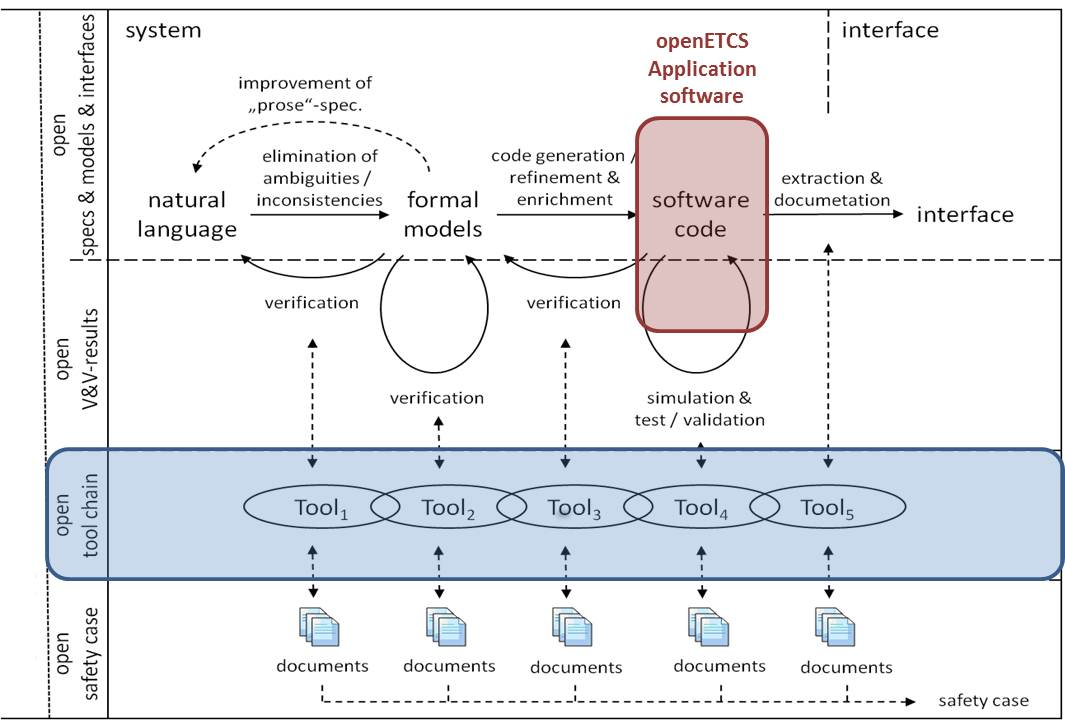
\includegraphics[width=16cm]{openETCS1}
  \caption{"open Proofs" the holistic approach}
  \label{fig:openETCS1}
\end{figure}


\section{openETCS tools chain}
The openETCS tools chain covers the entire software development process of the ETCS OBU,
starting from a conventional natural language specification over a formalization of the system
description for the modeling with verification steps, through to tool based code generation
and automatic generation of documents, see Figure \ref{fig:openETCS1}.
\\


\section{openETCS application software}
Software code generated from formal models, see Figure \ref{fig:openETCS1} above.\\



\section{Common terms and definitions}
\begin{table} [h]
\begin{tabular}{|p{2cm}|p{9cm}|p{3cm}|}
\hline
\bfseries Terms & \bfseries Definition & \bfseries Source \\ 
\hline 
\hline
formal specification  & A formal specification is a concise description of the behavior and properties of a system written in a mathematically-based language, specifying what a system is supposed to do as abstractly as possible, thereby eliminating distracting detail and providing a general description resistant to future system modifications. The most formal specifications are written in a language with a well-defined semantics that supports formal deduction and allows the consequences of the specification to be calculated through proof of putative theorems. & \cite{FM-doc}\\ 
\hline
formal proof  & A formal proof is a complete and convincing argument for the validity of a statement about a system description. A proof proceeds in a series of steps, each of which draws conclusions from a set of assumptions. Justification for each step is derived from a small set of rules which state what conclusions can be reasonably drawn from assumptions. Such justification eliminates ambiguity and subjectivity from the argument. Formal proofs may be prepared manually or, preferably, with the assistance of an automated FM tool. & \cite{FM-doc}\\ 
\hline
Open-Source-Software & Source code available to the general public with relaxed or non-existent copyright restrictions & EN 50128:2011 \\ 
\hline
Pre-existing software & All software developed prior to the application currently in question is classed as pre-existing software including: 
\begin{itemize}
\item COTS (commercial off-the-shelf) and open source software,
\item Software previously developed.
\end{itemize} & EN 50128:2011 \\ 
\hline
Open Proofs & An "open Proofs" is software or a system where all of the following are free-libre / open source software (FLOSS): 
\begin{itemize}
\item the entire implementation,
\item automatically-verifiable proof(s) of at least one key property, and,
\item required tools (for use and modification).
\end{itemize} & www.openproofs.org \\ 
\hline
Software & Intellectual creation comprising the programs, procedures, rules, data and any associated documentation pertaining to the operation of a system & EN 50128:2011 \\ 
\hline
Application software & Part of the software of a programmable electronic system that specifies the functions that perform a task related to the EUC rather than the functioning of, and services provided by the programmable device itself & IEC 61508-4:2010 \\ 
\hline
\end{tabular}
%\hline
\\
\caption{Terms and definitions}
\end{table}


\chapter{Introduction and motivation}
In all over Europe there are about 30 different, mostly not compatible signaling and train protection systems in use, see Figure \ref{fig:openETCS2}. For a unified european rail system it is very costly to maintain this diversity of signaling systems and therefore the european commission has set new rules by so called Technical Specifications for Interoperability (TSI, see the latest decision \cite{TSI-doc}) with the goal to implement a unified "European Train Control System (ETCS)".


\begin{figure}
\centering
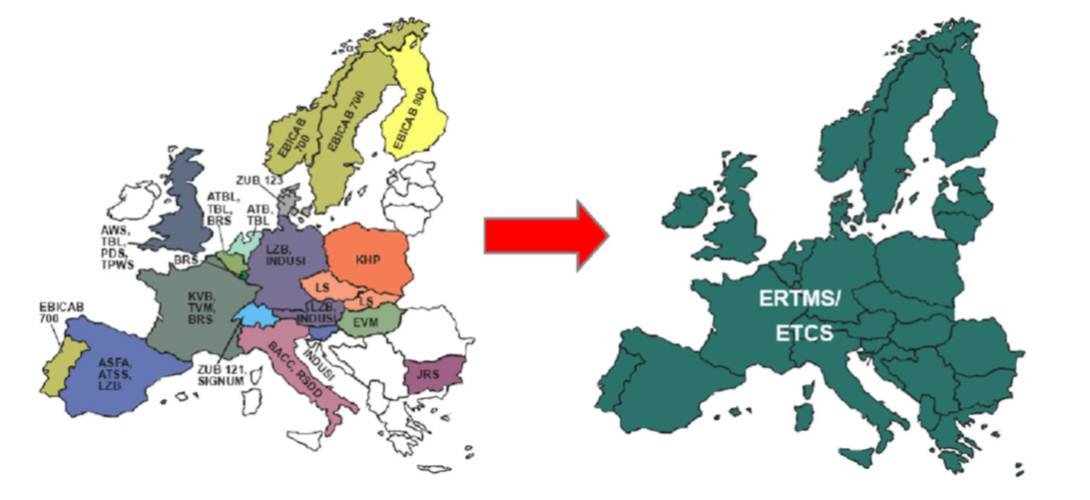
\includegraphics[width=12cm]{openETCS2}
\caption{Substitution of approximately 30 different signaling and ATP systems by just one single system: the European Train Control System (ETCS)}
\label{fig:openETCS2}
\end{figure}

ETCS is intended to replace national legacy signaling and train control systems and consists of facilities in the infrastructure and on-board units (OBU). ETCS is a so called cab-signaling system, which means that in principle all commands for the driver are shown on screens inside the driver's cabin, making conventional track-side signals obsolete, resulting in considerable savings for the infrastructure operators. The shift of functionality and safety responsibilities from the infrastructure into the vehicle has caused an increase of complexity for the on-board equipment. In terms of technology, this migration is mostly done by software. While electronic hardware is getting continuously cheaper, the high complexity of the safety critical software has caused significant cost increases for development, homologation and maintenance of the ETCS.
Despite the fact that several major European suppliers with substantial knowledge in signaling technology have worked on a common System Requirement Specification (SRS, see the latest baseline \cite{SRS-doc} ) for over a decade, the main goal of interoperability has not yet been accomplished. Up to now, not a single ETCS onboard unit has been approved to operate on all existing European ETCS lines. One of the reasons is given by the fact that a plain English specification text "prose" of some complexity cannot be so precise and free of potential divergent interpretation that the resulting software products would behave identical, see Figure \ref{fig:openETCS3}. Therefore the development of ETCS has to be considered as "work in progress", resulting in many software upgrades to be expected in the near and distant future.



\begin{figure}[h]
\centering
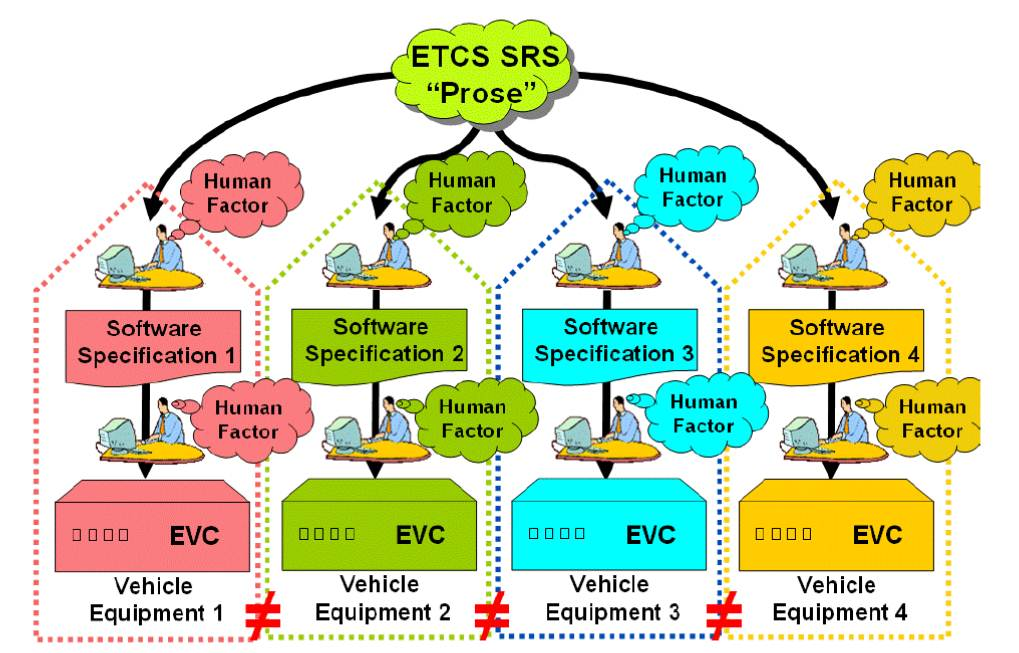
\includegraphics[width=1.0\textwidth, height=240px]{openETCS3}
\caption{Divergent interpretation of a common and mandatory public domain ETCS SRS document, due to the "human factor" by parallel working, not closely cooperating manufacturers, causing different software solutions with deviant reaction patterns, which results in interoperability deficiencies and costly subsequent retrofit works}
\label{fig:openETCS3}
\end{figure}

Almost all products on the market are based on different proprietary software designs, which results in a life-long dependency from the original manufacturers causing high life-cycle costs for vehicle owners. The key element for improving that situation seems to be a greater degree of standardization for: Hardware, software, methods and tools.
An approach following the open source idea, called "openETCS" utilizing concepts from the automotive and
aviation industry, has been suggested, not only covering the embedded application software of the ETCS onboard unit itself, but including all tools and documents in order to make the entire product life cycle as transparent as possible and make it comprehensible for third parties.
Making the proof of safety open to the public has been called "open proof" and is new to the railway sector, see Figure \ref{fig:openETCS4}.

\begin{figure}[h]
\centering
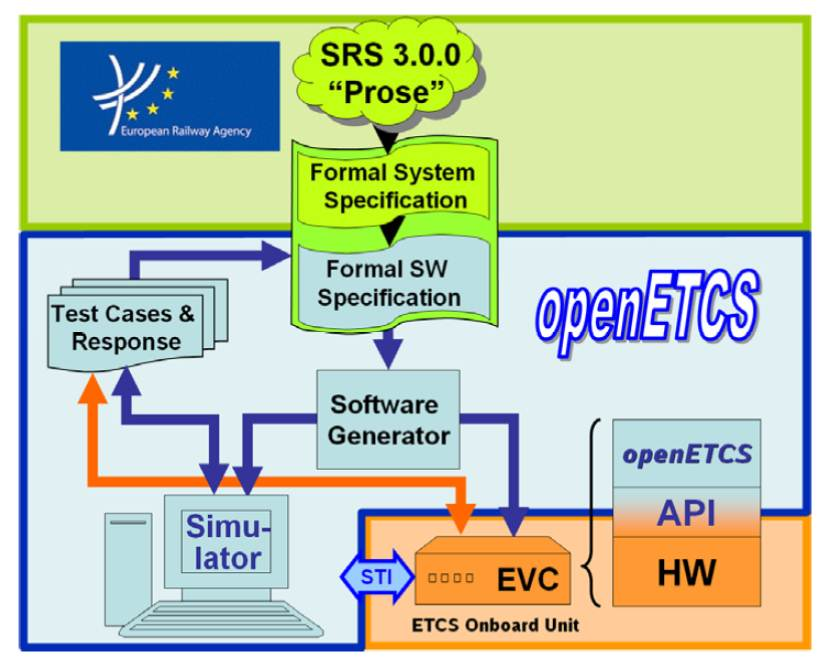
\includegraphics[width=1.0\textwidth, height=242px]{openETCS4}
\caption{openETCS approach}
\label{fig:openETCS4}
\end{figure}


\chapter{What is openETCS?}

\section{Description}
A detailed description of the project openETCS is given in the Project Outline Full Project
Proposal, see \cite{FPP13}.

\section{Main goals and deliverables}
The objective of the openETCS project is to provide a usable open source application software; including tools, documentations and the safety case for all ETCS OBU. That means, are made available as FLOSS under a "General Public License" (e.g. EUPL: European Union Public License).
\\
According to the project co-operation agreement \cite{PCA12}, the main goals and deliverables of the openETCS project are:
\begin{enumerate}
  \item Create a formal specification of the ETCS OBU functionality according to UNISIG Subset 026,
  \item Generate an executable software package from the formal specification and integrate the generated software package in the target hardware (non vital integration) for laboratory test, simulation and reference purposes,  
  \item Develop a tools chain supporting both previous bullet points including: code, test case and document generation, meeting CENELEC EN 50128:2011 requirements and certifiable for SIL4 software applications for signalling equipment.
\end{enumerate}


\chapter{Purpose and creation of this report}

\section{Purpose of this report}
Due to the particularity of this project and taking into account the goals of this project, it should be clarified in advance which requirements shall be fulfilled in order to be compliant with the CENELEC standard EN 50128:2011. The work was carried out and coordinated by AEbt and the result is this report. Hence, this report elicits requirements that must be fulfilled in order to prove, that the openETCS project deliverables are fit for theirs intended purpose and responds correctly to safety issues that was derived from the ERTMS System Safety Requirements Specification.

\section{Creation of this report}
\label{report}
Basis for the realisation of this report were:
\begin{itemize}
  \item Articles and other technical literature
  \item Existing processes in the signalling industry
  \item CENELEC standards
\end{itemize}

This work was also carried out through interviews with experts. The experts interviewed were industrial experts, signalling experts and standardisation experts. 


\chapter{Results}

This section describes the result of the performed work.

\section{Safety requirements to be fulfilled according to EN 50128:2011}

Safety requirements according to the CENELEC standard EN 50128:2011 that shall be fulfilled by the openETCS tools chain and the openETCS application software, are recorded in annex \ref{annexA} and \ref{annexC}.


\section{Security requirements to be fulfilled}

Security Requirements are not described in the standard EN 50128:2011, nevertheless due to the nature of this project and based on interviews performed with software and signalling experts, we recommend to take into account the recommendations described in sections \ref{DPatterns}, \ref{CPatterns} and \ref{Backdoor}.\\
Sections \ref{DPatterns1}, \ref{CPatterns1} and \ref{Backdoor1} give a brief description on familiar security patterns. A detailed description on all existing security patterns is given in \cite{SECU-doc}.

\subsection{Secure Design Patterns}
\label{DPatterns1}
During the design of the openETCS application software, software security can be enhanced through the implementation of secure design patterns. 
Three of the most techniques used are listed below:
\begin{enumerate}
  \item Distrustful decomposition
  \item Privilege separation
  \item Clear sensitive information
\end{enumerate}

\subsubsection{Distrustful decomposition}
The intent of the Distrustful Decomposition secure design pattern is to move separate functions into mutually untrusting programs, thereby reducing:
\begin{itemize}
  \item the attack surface of the individual programs that make up the system
  \item the functionality and data exposed to an attacker if one of the mutually untrusting programs is compromised
\end{itemize}

\subsubsection{Privilege separation}
The intent of the Privilege separation is to reduce the amount of code that runs with special privilege without affecting or limiting the functionality of the program. The Privilege separation is a more specific instance of the distrustful decomposition.

\subsubsection{Clear sensitive information}
The use of this pattern ensures that sensitive information is cleared from reusable resources before the resource may be reused. It is possible that sensitive information stored in a reusable resource may be accessed by an unauthorized user or adversary if the sensitive information is not cleared before freeing the reusable resource.


\subsection{Secure coding Patterns}
\label{CPatterns1}
During the implementation of the openETCS application software and tool chain, software security can be augmented by avoiding a number of common software security vulnerabilities. 
The following software security vulnerabilities shall be avoided:
\begin{enumerate}
  \item Buffer overflow
  \item Pointer shenanigans
  \item Dynamic memory allocation flaws
  \item Tainted data
\end{enumerate}

\subsubsection{Buffer overflow}
Buffer overflow can lead to more serious consequences, such as stack smashing, code injection, or even arc injection by which an attacker changes the control flow of the program by modifying the return address on stack. In arc injection, an attacker doesn't even have to inject any code, and he can jump to an arbitrary function in existing code, or bypass validity checks or assertions \cite{Kalinsky09}.

\subsubsection{Pointer shenanigans}
If an attacker can modify a data pointer, then the attacker can point to wherever he likes and write whatever he likes. If an attacker can overwrite a function pointer, the attacker is well on his way to executing his code on the processor \cite{Kalinsky09}.

\subsubsection{Dynamic memory allocation flaws}
The use of dynamic memory allocation shall be forbidden within the openETCS project. It is so easy to write defective code for dynamic memory allocation, so that attackers are eager to search out these defects \cite{Kalinsky09}.

\subsubsection{Tainted data}
Data entering an embedded system from the outside world must not be trusted. Instead, it must be "sanitized" before use \cite{Kalinsky09}.
A useful technique for data sanitization is called "white listing". It involves describing all possible valid values for a given piece of data and then writing code that only accepts those values. All unexpected values are viewed as "tainted" and are not used.

\subsection{Backdoor}
\label{Backdoor1}
A backdoor can be created by each person who has access to the software source code, but it is also possible to create a backdoor without modifying the software source code, or even modifying it after compilation. This can be done by rewriting the compiler so that it recognizes code during compilation that triggers inclusion of a backdoor in the compiled output. When the compromised compiler finds such code, it compiles it as normal, but also inserts a backdoor. This attack was first outlined by Ken Thompson in his paper "Reflections on Trusting Trust" \cite{Ken84}.
A useful technique against back doors is the so called "Diverse Double-Compiling"-technic see \cite{Wheeler09}. 


\section{Recommendation for the openETCS project}

\subsection{Regarding Secure design Patterns}
\label{DPatterns}
The architecture and design specification of the openETCS application software shall implement the requirements described in section \ref{DPatterns}.

\subsection{Regarding Secure coding Patterns}
\label{CPatterns}
Since the software code of the openETCS application software will be automatically generated using tools,  tools used or developed shall avoid the software security vulnerabilities described in section \ref{CPatterns}.

\subsection{Regarding Backdoors}
\label{Backdoor}
Experiences from the past have shown that open source software are better positioned against backdoors than proprietary software. For this reason, it is clear from the report of the European Parliament, that: "Calls on the Commission and Member States to promote software projects whose source text is made public (open-source software), as this is the only way of guaranteeing that no backdoors are built into programmes" see \cite{EUParl}.
Since openETCS is an open source software project and according to \cite{EUParl}, no requirement regarding backdoor issues need to be considered.


\section{Requirements regarding Hardware, operating system and the bus system}
When developing software, it is mandatory to prove that the actual behavior of the software, when executed, will be consistent with the behavioral semantics of the software. 
Behavior is observable in: 
\begin{itemize}\itemsep=0pt
  \item The data domain,
  \item The time domain,
  \item The causal domain.
\end{itemize}

All of these behavioral aspects depend on both the OS and the underlying HW \cite{BraPeFe12}:
\begin{itemize}\itemsep=0pt
  \item Data transformations fail if, for example, the word length of the HW registers is inappropriate for the calculations involved.,
  \item Expected reactions miss their deadlines if, for example, the OS scheduler does not allocate appropriate amounts of CPU time to the task processing the input,
  \item Events occur in the wrong order if the OS does not provide adequate mechanisms for critical section management.
\end{itemize}

As a consequence the openETCS application software can only be validated and certified in relation to certain OS and HW capabilities.
We therefore expect that the EVC code generated from the openETCS models will reference the interface of some OS application program interface (API) providing the services necessary to ensure the proper behavior of the software to be executed. Moreover, a list of hardware capabilities to be fulfilled has to be specified. 
We propose to elaborate specification documents about OS and HW capabilities required. 

The OS specification document should specify:
\begin{itemize}\itemsep=0pt
  \item the API required by the openETCS application software (Since the openETCS application software shall be SIL4 compliant, the required API shall also be SIL4 compliant according to EN 50128, see \cite{EN50128}),
  \item the scheduling capabilities (e.g., reaction to interrupts, partitioning in the time domain),
  \item the communication interfaces supported (It is expected that the System in which the openETCS application software will be implemented, will exchange safety-related signals with its environment, therefore, a risk analysis on the basis of EN 50126 and EN 50129 shall be performed to determine the SIL (Software-SIL) of the communication interface. However, it should be noted that the communication interfaces shall fulfill the requirements of EN 50159, see \cite{EN50159}).
\end{itemize}

Instead of specifying OS properties from scratch we suggest to adopt the well known OS specification from the ARINC 653 standard see \cite{ARINC} for which OS have been developed and are applied successfully for safety-critical tasks in the avionic domain.

The HW specification should include:
\begin{itemize}\itemsep=0pt
  \item The required HW architecture (Since the openETCS application software shall be SIL4 compliant, the required HW shall also be SIL4 compliant according to EN 50129, see \cite{EN50129}),
  \item The required HW interfaces and their performance characteristics,
  \item The CPU architecture (number of cores, word length etc.),
  \item Partitioning requirements (the need of a memory management unit),
  \item Existence of real time clocks.
\end{itemize}


\section{Is "open proofs" suitable for safety railway applications?}
As mentioned in section \ref{common-terms}; a software or system is an "open proof" if all of the following are FLOSS: 
\begin{enumerate}
\itemsep=0pt
  \item the entire implementation (requirements, design, code, required documentation for use/maintenance, etc.),
  \item automatically-verifiable proof(s) of at least one key property, and
  \item all required tools needed for use and modification of the software or system.
\end{enumerate}

According to (http://www.openproofs.org), something is FLOSS if it gives anyone the freedom to use, study, modify, and redistribute modified and unmodified versions of it, meeting the free software definition and the open source definition.

In a globally meaning, "open Proofs" embraces two approaches: formal methods and the freely availability of the software or system to others (in this report referred as open source).

\subsection{Suitability of open source process for safety relevant railway applications}
By order of the Deutsche Bahn AG (DB AG), AEbt has created an assessment report on the suitability of open source software for safety relevant railway applications.
In this Report, the assessor came to the conclusion that open source software regarding their safety integrity should be treated just as proprietary software. In certain areas, the use of open source software for safety relevant applications is even recommended; because software bugs or intentionally programmed backdoor will be early detected by independent programmers or the "community", see \cite{AEbt-doc}.


\subsection{Suitability of formal methods for safety relevant railway applications}
This section provided general information of the impact of introducing and integrating formal methods (FM) into the development process.

Formal methods for developing software embrace two techniques: formal specification and formal verification. Both are established based on elementary mathematics, such as set of theory, logic and algebraic theory \cite{SOFL-doc}.

When establishing formal methods on a project, there are basically two types of considerations, one of which is largely administrative, the other largely technical, \cite{FM-doc}. 

A summary of the each appears below.

\textbf{Administrative Factors:}
\begin{itemize}\itemsep=0pt
  \item \textbf{Project Staffing:} The team responsible for planning the role of FM on a project should include at least one person knowledgeable in FM and one person knowledgeable about the application domain. The team responsible for applying FM must have FM expertise or be provided with hands-on training.
  \item \textbf{Project Scale:} The scale of the project should be taken into consideration. If project staff has little or no previous FM experience, an initial study may be advisable either as a final objective or as a leading to the full-scale project.
  \item \textbf{FM Training:} The training available to those project staff responsible for applying FM should be rigorous and include hands-on experience with the tool(s) and type of application that will be encountered on the project.
  \item \textbf{Process Integration:} The strategy for integrating FM into a new or existing process should be thoroughly planned and documented, preferably early in the project.
  \item \textbf{Project Guidelines:} Project guidelines, standards, and conventions, both for documentation and specification, should be developed early and adhered to.
\end{itemize}

\textbf{Technical Factors:}
\begin{itemize}\itemsep=0pt
  \item \textbf{Type of Application:} FM are not equally appropriate for all applications; they are best suited to analyzing complex problems, taken singly and in combination, and less suited for numerical algorithms or highly computational applications..
  \item \textbf{Size and Structure of Application:} The size and structure of an application determine the difficulty of using FM; ideally, applications should be of moderate size (guidance on how to assess size will be addressed in this item's section below), decomposable into subsystems or components, and based on a coherent underlying structure.
  \item \textbf{Type of Analysis/Formal Method:} The type of analysis, i.e., the reasons for applying FM, determine the most appropriate level of formalization and the most suitable FM and FM tools. Objectives in using FM range from producing clear, unambiguous documentation to mechanically verifying the correctness of crucial algorithms or components.
  \item \textbf{Levels of Rigor in FM:} FM may be applied at varying levels of rigor. The rigor, or extent to which a method is "truly formal" and "really calculates," can range from the occasional appearance of mathematical notation in an otherwise informal document, through "rigorous" methods that employ a standardized specification language, to "fully formal" methods that make use of mechanically-checked theorem proving.
  \item \textbf{Scope of Formal Method Use:} There are at least three dimensions to the scope of formal method use: (1) all/selected stages of development life cycle, (2) all/selected system components, (3) full/selected (system) functionality.
  \item \textbf{Type of Formal Method Tool:} The choice of FM tool, if any, should be directly determined by the application profile generated by evaluating the five preceding factors. Primary considerations include the type of specification language and the need for mechanical proof support.
\end{itemize}

Administrative and technical considerations are closely coupled, each having implications for the other. This is because the process of determining whether a given application is a good candidate for FM is not cut and dried and because the use of FM entails a serious technical commitment by project staff and a corresponding commitment to support and invest in the FM activity on the part of management. 


\subsubsection{Detailed description of the technical considerations}
Formal methods cover a wide range of techniques that have different characteristics and utility. This section describes the scope and implications of these differences with respect to five technical factors that should be evaluated when considering the use of FM for a given application. The factors are introduced in the suggested order of consideration (according to \cite{FM-doc}); e.g., before choosing a formal method tool, it is important, first, to define the type and scope of application, second, to specify the type of analysis to be performed and third, to determine the rigor and scope of the analysis.

\textbf{Type of Application}
FM are not equally suitable for all types of applications. Although, in principle, the methods can be applied to nearly any application, in practice, the benefits that can be realized and the difficulty of achieving them will differ significantly from one application to another and from one subsystem to another within a single application. Suitability should be evaluated with respect to the characteristics of the problem domain and their implications for the modeling domain. 
Higher complexity applications stand to gain from FM much more than lower complexity ones simply because less complex problems can be solved dependably using less rigorous methods. Of particular interest are problem domains whose complexity stems not so much from the size and structure of the design, but from inherently difficult algorithms such as those for fault tolerance and parallel or distributed processes. 
A further consideration is the mathematical domain of discourse. Applications that are heavily based on numerical processing, especially those using floating point arithmetic, pose some difficulties for FM, while those that can be modeled using the domains of logic and discrete mathematics benefit from easier formalization, more tractable reasoning, and better FM tool support.

\textbf{Size and Structure of Application}
The size of an application is a major factor in the cost and difficulty of its formalization. 
Usually, FM are most effectively applied to systems or subsystems of moderate size; currently, FM cannot be applied in full to the largest systems implementable using conventional programming techniques. An alternative is to limit the scope of the formal method activity to critical properties or components of a very large system, assuming, of course, that the system is decomposable into small or medium-sized subsystems or components with well-defined interfaces. This clean structuring property is vital in any medium- or large-scale application to ensure that the results of separate FM analyses can be combined and valid inferences drawn about the composite behavior of cooperating subsystems.
A second structural property, loosely referred to as structural entropy, is also important. If an application has intrinsically high entropy, i.e., is primarily a random collection of special cases with weak cohesion or few unifying principles, little can be expected from a formalization activity. Conversely, if an application exhibits strong underlying structural principles, well understood and easily expressed in a logically meaningful way, FM can effectively capture and exploit this structure.

\textbf{Type of Analysis/Formal Method }
The type of analysis or formal method to be employed is determined largely by project objectives; the purpose for which FM are to be applied should be clearly defined and explicitly documented. For example, one application may use FM primarily to develop specifications for documentation, another may exploit the precision inherent in formally specified requirements to catch errors early in the life cycle, a third may use FM to analyze and assure the correctness of critical properties or algorithms. These equally legitimate objectives have very different implications for the rigor of the formal method analysis and the type of formal method tool appropriate for the project.

\textbf{Levels of Rigor in Formal Methods }
FM techniques may be applied at varying levels of rigor. Here, rigor is used in a technical sense to mean the degree of formality of a method, i.e., the extent to which a method formulates specifications in an axiomatic style, explicitly enumerates all assumptions, and reduces proofs to explicit applications of elementary rules of inference. Increasing formality allows the products of FM (i.e., specifications and proofs) to be less dependent on subjective reviews and consensus and more amenable to systematic analysis and replication. Usually, increasing formality is associated with increasing dependence on mechanical support. Suggested levels of rigor according to \cite{FM-doc}
\begin{itemize}\itemsep=0pt
  \item \textbf{Level 1:} Use of manual review and inspection, relying on documents written in a natural language, pseudo code, or programming language, possibly augmented with diagrams and equations, and validated with conventional testing techniques. Activities at this level are not "formal" in a strict sense, but represent current recommended practice, and serve as a baseline of discipline and structure necessary to support the additional activities at higher levels of formality.
  \item \textbf{Level 2:} Use of notations and concepts derived from logic and discrete math to develop more precise requirements statements and specifications. Proof, if any, is informal. This level of FM typically augments existing processes without imposing wholesale revisions.
  \item \textbf{Level 3:} Use of formalized specification languages with mechanized support tools ranging from syntax checkers and pretty printers to type checkers. This level of formality usually includes support for modern software engineering constructs, e.g., modules, abstract data types, and objects, all with explicit interfaces, but has not historically offered mechanized theorem proving.
  \item \textbf{Level 4:} Use of fully formal specification languages with rigorous semantics and correspondingly formal proof methods that support mechanization. State exploration, model checking, and language inclusion technologies also exemplify this level, although these technologies are highly specialized, automatic theorem provers that are limited to checking properties of finite-state systems. 
\end{itemize}
Higher levels of rigor are not necessarily superior to lower levels; factors that determine the appropriate level of rigor include: project objectives, criticality of the application, and available resources. For example, if FM are used simply as documentation, Level 2 may be appropriate; if they are used to justify the design of a new and critical component, Level 4 may be the best choice. On the other hand, routine applications adequately handled by conventional processes are probably most appropriately left to Level 1. Finally, it is possible to use a formal method at a level of rigor lower than its ultimate capability, e.g., by using the specification language, but not the theorem-proving capability of a Level 4 formal method. 

\textbf{Scope of Formal Method Use}
The extent to which FM are applied can also vary. There are at least the following three dimensions to the notion of extent.
\begin{enumerate}\itemsep=0pt
  \item \textbf{All or selected stages of the development life cycle:} It is generally felt that the biggest payoff from the use of FM occurs in early life cycle stages, given that errors become more expensive to correct as they proceed undetected through later development stages; early detection leads to lower life cycle costs. Moreover, the use of FM in the early stages provides additional precision where it is currently most needed in the conventional development process.
  \item \textbf{All or selected system components:} Criticality assessments, assurance considerations, and architectural characteristics are among the key factors used to determine which subsystems or components to analyze with FM. Since large systems are typically composed of components with widely differing criticalities, the extent of formal method use should be dictated by project-specific criteria. For example, a system architecture that provides fault containment for a critical component through physical or logical partitioning provides an obvious focus for FM activity and enhances its ability to assure key system properties.
  \item \textbf{Full or selected system functionality:} Although FM have traditionally been associated with "proof of correctness," i.e., ensuring that a system component meets its functional specification, they can equally well be applied to only the most important system properties. Moreover, in some cases it is more important to ensure that a component does not exhibit certain negative properties or failures, rather than to prove that it has certain positive properties, including full functionality.
\end{enumerate}
These are the three most commonly used variations on the extent of FM application, although others are certainly possible. Varying the degree of rigor along each of these three dimensions yields a wide range of options and provides maximal benefit from a limited investment in FM.

\textbf{Type of Formal Method Tool}
The choice of tool is dictated by the application profile defined by consideration of all of the preceding factors, although the issue of tools is clearly moot if the most appropriate level of rigor falls below Level 3. For example, Level 3 documentation of sequential components is consistent either with a typical Level 3 notation supported by a type checker, or, if more powerful mechanization and stronger guarantees of consistency are desired, with a system normally used to support Level 4. Similarly, when choosing a Level 4 tool, the capability of the tool, the constraints of the problem domain, and the objectives of the analysis must be well matched. For example, verifying the correctness of fault-tolerant algorithms is probably best pursued with a general-purpose theorem prover, while exploring the properties of mode-switching or other complex control logic is probably more effectively pursued with a state-exploration system.
The process of selecting a formal method tool is in many ways similar to selecting any other software system; the usual considerations of documentation, tutorials, history of use, ease of use, etc. apply. In this case, effective support for the selected formal method(s) is also important. A suggestive, but by no means exhaustive, list of the additional considerations necessary for judicious tool selection appears below. 
\begin{enumerate}\itemsep=0pt
  \item \textbf{Specification Language:} Is the language adequately expressive for the given application and which of the following features important for the application does the language offer: well-defined semantics, modern programming language constructs (including support for abstraction, modularity, and encapsulation), familiar and convenient syntax, strong typing, encapsulation, parameterization, built-in model of computation, executable subset or other provision for animating specifications, support for state exploration, model checking, and related methods?
  \item \textbf{Theorem Prover:} Does the FM tool offer a theorem prover or proof checker? If so, how is the theorem prover controlled and guided; is there automated support for arithmetic reasoning, efficient handling of large propositional expressions, and rewriting; what support is there for developing and viewing the proof; how is the proof presented to the user (e.g., user input or canonical expressions, with or without quantifiers); are the foundations (i.e., all axioms, definitions, assumptions, lemmas) of the proof identified; are there facilities for editing proofs; is it reasonably easy to re-verify a theorem after slight changes to the specification?
  \item \textbf{Utilities:} Does the formal method offer a reasonably comprehensive library of standard types, functions, and other constructions and is the library validated; what, if any, editing and document preparation tools does the system provide; are there facilities for cross-referencing, browsing, and requirements tracing; is there support for incremental development across multiple sessions and for change control and version management?
\end{enumerate}


\subsection{Position of standards regarding formal methods in the railway sector}
In EN 50128:2011, Formal Methods/Proofs are explicitly identified as relevant technique/measure for software requirements specification, software architecture, software design, implementation, verification and testing and data preparation techniques. More precisely they are "recommended" for SIL levels 1 and 2 and "Highly Recommended" for SIL levels 3 and 4. The standard puts additional constraints on tools, especially code/data generation tools with respect to the need of a specification and evidence that the implementations complies with the specification. 
Unfortunately, formal methods have not spread in the whole railway signalling industries, where much software is still written and tested in traditional ways. This lack of adoption is due to the investments needed to build up a formal methods culture, and to the high costs of commercial support tools. Moreover, equipment can conform to CENELEC without applying formal methods \cite{Proc-doc}. 
Another barrier is that, the certification bodies might not be familiar with FM as most of the systems they certify follow a test-based approach. For systems whose justification relies on such formal argument, the certification body might require additional information to be convinced. Typically, one should foresee some specific training-level information in the certification process. Once acquired, new system can easily follow the same path. For example siemens has gone through this process with the B-method, and it is now accepted by the certification bodies, so that the next projects have become easier to certify. 

\textbf{In summary:} The EN 50128:2011 highly recommend formal methods but do not really describe how to manage a formal development. It is therefore difficult to prove that the development process comply with the standards. Certification authorities have to be convinced about this issue. 
As formal methods are less widespread and certification authorities are less familiar with them as compared to the classical development methods, there is more work to be done in comparison with other methods, especially the first time, and despite the fact that better argument could be provided. However the investment might be worth the effort as shown by the Siemens case for B. 


\chapter{Summary}
As task leader of the task D2.2 (according to \cite{FPP13}), AEbt has coordinated all the work. Basis, were the procedures listed in the section \ref{report} of this report. The result is a first set of requirements, which shall be fulfilled in order to assess tools of the openETCS tools chain as T1, T2 or T3 support tools according to EN 50128:2011. 
Regarding the openETCS application software, it was assumed during the creation of this document, that the whole or part of the software will be SIL4 compliant according to EN 50128:2011.

Requirements in appendix \ref{annexA} and \ref{annexC} with suggested implementation are general requirements that any SIL4 Software for railway applications and tools shall fulfill. For specific projects, there can still be minor deviations, which may have to be agreed with a software assessor.

Based on the performed assessment and interviews, we are of the opinion that "open proofs" is suitable for safety railway applications, when the process applied to develop, test, deploy and maintain the software or tools fulfills all the requirements of the CENELEC standard EN 50128:2011 as well as security requirements.

In this report reference was made to other standard; which however have not been addressed, see CENELEC EN 50159:2010 \cite{EN50159} and ARINC \cite{ARINC}.
Related to the standard ARINC \cite{ARINC}, an analysis shall be performed, in order to show, how it can be helpful for the openETCS project. Regarding the standard EN 50159:2010 \cite{EN50159}, we also recommend to perform an analysis, in order to find out which requirements from this standard and based on the allocated software SIL to the communication interface shall be implemented.





%\section{Aenean imperdiet}
%\lipsum[11]


\nocite{*}

\bibliographystyle{unsrt}
\bibliography{erdc}

\appendix

\chapter{\\Tools development: state of the art regarding CENELEC EN 50128:2011}
\label{annexA}

\section{Introduction}
This section gathers requirements, which shall be fulfilled by tools within the openETCS tools chain.
Since some of the tools of the openETCS tools chain not really need to be T3 compliant, the requirements to tools were therefore subdivided in 3 subsections:
\begin{itemize}\itemsep=0pt
  \item Section \ref{T1}, gathers requirements for tool in class T1,
  \item Section \ref{T2}, gathers requirements for tool in class T2 and,
  \item Section \ref{T3}, gathers requirements for tool in class T3.
\end{itemize}

\subsection{How to read the tables used in this section}
Tables used in this appendix consist of three columns.
\begin{itemize}\itemsep=0pt
  \item \textbf{Column 1} lists the requirements comming from the CENELEC standard EN 50128:2011. But since the standard is protected by copyright, only the requirements identification numbers are recorded there. The same requirements identification numbers (subclause) as defined in the EN 50128:2011 have been used. The textual requirement should therefore be read in the standard using the requirements identification number recorded in column 1 as reference.\\
In order to simplify the readability, some of the requirements have been grouped, especially when they address the same subject; only few were left out, because they were not relevant for the purpose.
  \item \textbf{column 2} describes how the various requirements can be fulfilled. Everywhere where possible, recommendations were formulated.
  \item \textbf{column 3} lists documents that shall be created or provided, in order to provide the evidence.
\end{itemize}



\section{Requirements for tools in class T1}
\label{T1}
Some examples of T1 tools:
\begin{itemize}\itemsep=0pt
  \item a text editor tool with no automatic code generation capabilities,
  \item a requirement support tool with no automatic code generation capabilities,
  \item a design support tool with no automatic code generation capabilities,
  \item configuration control tools.
\end{itemize}

{\footnotesize\sffamily\centering
\begin{longtable}{|p{2cm}|p{9cm}|p{3cm}|}
\caption{Requirements for tools in class T1}\\
\hline
\bfseries Requirements & \bfseries How the evidence shall be provided & \bfseries Documents to be created\\
\hline
\hline
\endhead
\hline
%\caption{Terms and definitions}
\endfoot

6.7.4.1 & Provide the evidence that tools in class T1 cooperate.
\linebreak
\linebreak
NOTE \linebreak
Tools cooperate if the outputs from one tool have suitable content and format for automatic input to a subsequent tool, thus minimizing the possibility of introducing human error in the reworking of intermediate results. & Evidence report for T1 tools.\\ 
\hline

\end{longtable}}



\section{Requirements for tools in class T2}
\label{T2}
Tools in class T2 are in general verification tools.\\
Some examples of T2 tools:
\begin{itemize}\itemsep=0pt
  \item static code analysers,
  \item test coverage monitors,
  \item theorem proving assistants,
  \item simulators and,
  \item model checkers.
\end{itemize}

{\footnotesize\sffamily\centering
\begin{longtable}{|p{2cm}|p{9cm}|p{3cm}|}
\caption{Requirements for tools in class T2}\\
\hline
\bfseries Requirements & \bfseries How the evidence shall be provided & \bfseries Documents to be created\\
\hline
\hline
\endhead
\hline
%\caption{Terms and definitions}
\endfoot

6.7.4.1 & Provide the evidence that tools in class T2 cooperate.
\linebreak
\linebreak 
NOTE \linebreak
Tools cooperate if the outputs from one tool have suitable content and format for automatic input to a subsequent tool, thus minimizing the possibility of introducing human error in the reworking of intermediate results. & Evidence report for T2 tools.\\ 
\hline
6.7.4.2 & Provide a justification report for the selection of tools in class T2.
\linebreak
\linebreak 
NOTE \linebreak
The justification report shall include the identification of potential failures which can be injected into the tools output and the measures to avoid or handle such failures. & Justification report for T2 tools.\\ 
\hline
6.7.4.3 & Provide a tool manual for each tool in class T2.
\linebreak
\linebreak
NOTE \linebreak
A manual which clearly defines the behaviour of the tool and any instructions or constraints on its use. & Tool Manual for each T2 tools.\\ 
\hline
6.7.4.10 & Each tool in class T2 must be subject to configuration management. & A configuration management process for tools in class T2 shall be defined.\\ 
\hline
6.7.4.11 & For each new version of tools in class T2 that is used, provide the evidence that the new version contains no significant new unknown faults. & Evidence report, when a new version of T2 tool class is used.\\ 
\hline
\end{longtable}}



\section{Requirements for tools in class T3}
\label{T3}
Some examples of T3 tools: 
\begin{itemize}\itemsep=0pt
  \item Design refinement tools,
  \item Compilers,
  \item Assemblers,
  \item linkers,
  \item binders,
  \item loaders,
  \item Code generation tools,
  \item Diagnostic tools used to maintain and monitor the software under operating conditions,
  \item Application data/algorithm tools.
\end{itemize}

{\footnotesize\sffamily\centering
\begin{longtable}{|p{2cm}|p{9cm}|p{3cm}|}
\caption{Requirements for tools in class T3}\\
\hline
\bfseries Requirements & \bfseries How the evidence shall be provided & \bfseries Documents to be created\\
\hline
\hline
\endhead
\hline
%\caption{Terms and definitions}
\endfoot

6.7.4.1 & Provide the evidence that tools in class T3 cooperate. 
\linebreak
\linebreak 
NOTE \linebreak
Tools cooperate if the outputs from one tool have suitable content and format for automatic input to a subsequent tool, thus minimizing the possibility of introducing human error in the reworking of intermediate results. & Evidence report for T3 tools.\\ 
\hline
6.7.4.2 & Provide a justification report for the selection of tools in class T3.
\linebreak
\linebreak 
NOTE \linebreak
The justification report shall include the identification of potential failures which can be injected into the tools output and the measures to avoid or handle such failures. & Justification report for T3 tools.\\ 
\hline
6.7.4.3 & Provide a tool manual for each tool in class T3.
\linebreak
\linebreak
NOTE \linebreak
A manual which clearly defines the behaviour of the tool and any instructions or constraints on its use. & Tool Manual for each T3 tools.\\ 
\hline
6.7.4.4 & Provide the evidence that the tools fulfill the requirements for tools in class T3.

According to EN 50128:2011, the evidence may be based on one of the following topic:
\begin{enumerate}\itemsep=0pt
  \item a suitable combination of history of successful use in similar environments and for similar applications6 (within the organisation or other organisations).
  \item a tool validation report as specified in 6.7.4.5.
  \item diverse redundant code which allows the detection and control of failures resulting in faults introduced by a tool.
  \item Compliance with the safety integrity levels derived from the risk analysis of the process and procedures including the tools.
  \item other appropriate methods for avoiding or handling failures introduced by tools
\end{enumerate}
%\linebreak
%\linebreak
& \textbf{Recommendation:} \linebreak
\linebreak
\textbf{For Tool in class T3, we highly recommend to develop them according to the requirements described in annex \ref{annexB}.}\\ 
\hline
6.7.4.5 & Provide or create a tool validation report as evidence for the safety integrity of tool in class T3 (refer to 6.7.4.4) .
\linebreak
\linebreak
NOTE \linebreak
The validation report as mentioned in 6.7.4.4 shall address the following topic:
\begin{itemize}\itemsep=0pt
  \item a description of the validation activities;
  \item the version of the tool manual being used;
  \item the tool functions being validated;
  \item tools and equipment used;
  \item the results of the validation activity;
  \item test cases and their results for subsequent analysis;
  \item discrepancies between expected and actual results.
\end{itemize}
& Tool validation report.\\ 
\hline
\end{longtable}}


\chapter{\\Development process for tools in class T3}
\label{annexB}

\section{Introduction}
This appendix describes the development process for tools in class T3.\\
The process described in this appendix is only a suggestion, because the standard CENELEC EN 50128:2011 describes several ways to prove the safety integrity of a T3 tool. The process described in this appendix may be a complex development process, but it offers the advantage that the assessment process is structured and less complex.\\
The process described in this appendix is a mapping of the development process for SIL4 software according to the CENELEC standard EN 50128:2011.



\section{Boundary conditions for operating systems and hardware (Clause 4 according to EN 50128:2011)}
{\footnotesize\sffamily\centering
\begin{longtable}{|p{2cm}|p{9cm}|p{3cm}|}
\caption{Boundary conditions for operating systems and hardware (Clause 4 according to EN 50128:2011)}\\
\hline
\bfseries Requirements & \bfseries How the evidence shall be provided & \bfseries Documents to be created\\
\hline
\hline
\endhead
\hline
%\caption{Terms and definitions}
\endfoot

4.1 & specify the capabilities and boundary conditions to be fulfilled by the operating system and hardware. 
& Boundary conditions for the operating system and hardware.\\ 
\hline
\end{longtable}}


\section{Management and organisation (Clause 5 according to EN 50128:2011)}
\label{clause5}
\subsection{Management and organisation}
The objective of this subclause is to ensure that all personnel who have responsibilities within the development of the tools are organised, empowered and capable of fulfilling their responsibilities.
{\footnotesize\sffamily\centering
\begin{longtable}{|p{2cm}|p{9cm}|p{3cm}|}
\caption{Management and organisation regarding the development tools in class T3 (Subclause 5.1 according to EN 50128:2011)}\\
\hline
\bfseries Requirements & \bfseries How the evidence shall be provided & \bfseries Documents to be created\\
\hline
\hline
\endhead
\hline
%\caption{Terms and definitions}
\endfoot

5.1.2.1 & An EN ISO 9001 certification for each organisation involved in the tool development process is highly recommended & EN ISO 9001 certification or Evidence of a quality management process according to EN ISO 9001.\\ 
\hline
5.1.2.2, 5.1.2.3 and 5.1.2.9 to 5.1.2.14 & Create a quality assurance plan for the tool development process. 
\linebreak
\linebreak
\textbf{NOTE }
\begin{itemize}\itemsep=0pt
  \item The quality assurance plan shall be written according to subclause 6.5.
  \item The quality assurance plan shall also implement the requirements of 5.1.2.2, 5.1.2.3, 5.1.2.9, 5.1.2.10, 5.1.2.13 and 5.1.2.14.
\end{itemize}
& Quality assurance plan for the tool development process\\ 
\hline
5.1.2.4 to 5.1.2.8 & Create an assessment plan for the tools. (only when required).
& Assessment Plan for the tool development process\\ 
\hline
\end{longtable}}

\subsection{Personnel Competence}
\begin{flushleft}
The objective of this subclause is to ensure that all personnel who have responsibilities for the development of tools are competent to discharge those responsibilities by demonstrating the ability to perform relevant tasks correctly, efficiently and consistently to a high quality and under varying conditions.
\end{flushleft}
{\footnotesize\sffamily\centering
\begin{longtable}{|p{2cm}|p{9cm}|p{3cm}|}
\caption{Personnel competence regarding tools in class T3 (Subclause 5.2 according to EN 50128:2011)}\\
\hline
\bfseries Requirements & \bfseries How the evidence shall be provided & \bfseries Documents to be created\\
\hline
\hline
\endhead
\hline
%\caption{Terms and definitions}
\endfoot

5.2.2.1 and 5.2.2.2 & After it has been named and recorded in the quality assurance plan who is:
\begin{itemize}\itemsep=0pt
  \item Requirements Manager,
  \item Designer,
  \item Implementer,
  \item Tester,
  \item Verifier,
  \item Integrator,
  \item Validator,
  \item Project Manager,
  \item Configuration Manager.
\end{itemize}
and what their responsibilities within the tool development process are, now it shall be proved, that these persons are competent to discharge these responsibilities.

We propose to create a kind of "openETCS people competence matrix" at the management level. 

In this document the CV of all persons involved in the project must be recorded.
Where key competencies to fulfill a role are miss-ing, trainings must be provided.
Participation in trainings shall also be recorded in this document.
& openETCS people competence matrix
\linebreak
\linebreak
NOTE\linebreak
the created people competence matrix can also be used as evidence for the development process of the openETCS application software\\ 
\hline
5.2.2.3 and 5.2.2.4 & See requirement 5.1.2.1 & EN ISO 9001 certification or Evidence of a quality management process according to EN ISO 9001.\\ 
\hline
\end{longtable}}

\subsection{Lifecycle issues and documentation}
\label{SDLC}
\begin{flushleft}
The objective of this subclause is to structure the development of tools into defined phases and activities and to record all informations throughout the lifecycle.
\end{flushleft}
{\footnotesize\sffamily\centering
\begin{longtable}{|p{2cm}|p{9cm}|p{3cm}|}
\caption{Lifecycle issues and documentation regarding tools in class T3 (Subclause 5.3 according to EN 50128:2011)}\\
\hline
\bfseries Requirements & \bfseries How the evidence shall be provided & \bfseries Documents to be created\\
\hline
\hline
\endhead
\hline
%\caption{Terms and definitions}
\endfoot

5.3.2.1 and 5.3.2.3 & Select a lifecycle model for the development of tools.
& The selected lifeycle model shall be described in the \textbf{tool quality assurance plan}.\\ 
\hline
5.3.2.2 & See requirement 5.3.2.14 & See requirement 5.3.2.14\\ 
\hline
5.3.2.4 & \textbf{The Quality Assurance Plan}, \textbf{Verification Plan}, \textbf{Validation Plan} and \textbf{Configuration Management Plan} shall be drawn up at the start of the project and maintained throughout the development life cycle of the tools & Recommendation\\ 
\hline
5.3.2.5 & 
\begin{itemize}\itemsep=0pt
  \item Define all the activities to be performed at each phase of the tool development lifeycle model,
  \item Create planning documents at the project start
\end{itemize} 
& Planning documents\\ 
\hline
5.3.2.6 and 6.5.4.9 & Define a document management process for the tool development process.
\begin{itemize}\itemsep=0pt
  \item The process shall be described in a document management plan,
  \item The created document management plan shall implement requirements of 5.3.2.6 and 6.5.4.9.
\end{itemize}
& Document management plan for the tool development process\\ 
\hline
5.3.2.7 & Create an overall notation for documents, create a documents relationship matrix
& 
- Overall notation for documents 

- Documents relationship matrix for the tool development process.
\linebreak
\linebreak
Both documents shall be referenced in the tool quality assurance plan\\ 
\hline
5.3.2.8 and 5.3.2.10 & Create an overall definition of terms and abbreviations to be used for the tool development process. 

The created "overall definition of terms and abbreviations" shall implement requirements 5.3.2.8 and 5.3.2.10
& Overall definition of terms and abbreviations.
\linebreak
\linebreak
NOTE\linebreak
The created document shall be referenced in the tool quality assurance plan.\\ 
\hline
5.3.2.9 & Create a checklist to verify the internal consistency of each created documents during the development of the tools.


The created checklist shall implement the requirement 5.3.2.9.
& Checklist to verify the internal consistency of documents.
\linebreak
\linebreak
NOTE\linebreak
The created Checklist shall be referenced in the tool quality assurance plan.\\ 
\hline
5.3.2.11 & Use well-established document file formats (html, ps, pdf, rtf, odf or latex).
& The selected file formats shall be recorded in the tool quality assurance plan.\\ 
\hline
5.3.2.12 and 5.3.2.13 & We do not recommend to combine documents created by independent roles. 
& - \\ 
\hline
5.3.2.14 & Where any alternative lifecycle or documentation structure is adopted, provide the evidence that it meets all the objectives and requirements of the CENELEC EN 50128:2011.
\linebreak
\linebreak
NOTE\linebreak
The Evidence may be based on the following topic:
\begin{itemize}\itemsep=0pt
  \item top-down design methods,
  \item modularity,
  \item verification of each phase of the development lifecycle,
  \item verified components and component libraries,
  \item clear documentation and traceability,
  \item auditable documents,
  \item validation,
  \item configuration management and change control and
  \item appropriate consideration of organisation and personnel competency issues.
\end{itemize}
& Proof report, when any alternative lifecycle or documentation structure is adopted.\\ 
\hline
\end{longtable}}



\section{Quality assurance measures (Clause 6 according to EN 50128:2011)}
\label{clause6}
\subsection{Testing activities}
\begin{flushleft}
The objective of this subclause is to ascertain the behaviour or performance of the developed tool against the corresponding test specification to the extent achievable by the test coverage.
\end{flushleft}
{\footnotesize\sffamily\centering
\begin{longtable}{|p{2cm}|p{9cm}|p{3cm}|}
\caption{Testing activities during the development of tools in class T3 (Subclause 6.1 according to EN 50128:2011)}\\
\hline
\bfseries Requirements & \bfseries How the evidence shall be provided & \bfseries Documents to be created\\
\hline
\hline
\endhead
\hline
%\caption{Terms and definitions}
\endfoot

6.1.4.1 to 6.1.4.4 and 8.4.8.6 & Created Test Specifications. 
Each created Test Specification shall implement the requirement of 6.1.4.4 and 8.4.8.6.
& Test Specifications for tools\\ 
\hline
6.1.4.5 & Created test report. 
Each created test report shall implement the requirement of 6.1.4.5.
& Test Reports for tools\\ 
\hline
\end{longtable}}


\subsection{Verification activities}
\begin{flushleft}
The objective of this subclause is to examine and arrive at a judgment based on evidence that output items (process, documentation, software) of a specific development phase fulfill the requirements and plans with respect to completeness, correctness and consistency.
\end{flushleft}
{\footnotesize\sffamily\centering
\begin{longtable}{|p{2cm}|p{9cm}|p{3cm}|}
\caption{Verification activities during the development of tools in class T3 (Subclause 6.2 according to EN 50128:2011)}\\
\hline
\bfseries Requirements & \bfseries How the evidence shall be provided & \bfseries Documents to be created\\
\hline
\hline
\endhead
\hline
%\caption{Terms and definitions}
\endfoot

6.2.4.1 to 6.2.4.9 and 8.4.8.6 & Create a verification plan.

The created verification plan shall implement the requirement of 6.2.4.9 and 8.4.8.6.
\linebreak
\linebreak
NOTE: \linebreak
For verification activities, appropriate combinations of techniques for software SIL4 as described in annex A, table A.5, A,6, A.7 and A.8 of EN 50128:2011 shall be selected and recorded in the tool verification Plan.
& verification plan for tools\\ 
\hline
6.2.4.10 to 6.2.4.11 & verify the created verification plan for tools. 
\begin{itemize}\itemsep=0pt
  \item The results of the verification shall be recorded in the quality assurance verification report,
  \item The created quality assurance verification report shall implement the requirements of 6.2.4.11. 
\end{itemize}
& Quality assurance verification report for tools.\\ 
\hline
6.2.4.12 to 6.2.4.13 & Create verification reports.

Each created verification report shall implement the requirements of 6.2.4.13.
& Verification Reports for tools.\\ 
\hline
\end{longtable}}



\subsection{Validation activities}
\begin{flushleft}
The objective of this subclause is to determine whether the developed tool fits the user needs, in particular with respect to safety and quality and with emphasis on the suitability of its operation in accordance to its purpose in its intended environment.
\end{flushleft}
{\footnotesize\sffamily\centering
\begin{longtable}{|p{2cm}|p{9cm}|p{3cm}|}
\caption{Validation activities during the development of tools in class T3 (Subclause 6.3 according to EN 50128:2011)}\\
\hline
\bfseries Requirements & \bfseries How the evidence shall be provided & \bfseries Documents to be created\\
\hline
\hline
\endhead
\hline
%\caption{Terms and definitions}
\endfoot

6.3.4.1 to 6.3.4.6 and 8.4.8.6 & Create a validation plan.

The created validation plan shall implement the requirements of 6.3.4.4 and 8.4.8.6.
& Validation Plan for tools\\ 
\hline
6.3.4.7 to 6.3.4.11 & Create a validation report.

The created validation report shall implement the requirements from 6.3.4.8 to 6.3.4.11
& Validation report for tools.\\ 
\hline
6.3.4.13 & verify the created validation plan for tools. 
\begin{itemize}\itemsep=0pt
  \item The results of the verification shall be recorded in the validation verification report,
  \item The created validation verification report shall implement the requirements of 6.3.4.13. 
\end{itemize}
& Validation plan verification report for tools.\\ 
\hline
6.3.4.14 & verify the created validation report for tools. 
\begin{itemize}\itemsep=0pt
  \item The results of the verification shall also be recorded in the validation verification report,
  \item The created validation verification report shall also implement the requirements of 6.3.4.14. 
\end{itemize}
& Validation verification report for tools.\\ 
\hline
\end{longtable}}


\subsection{Assessment activities}
These activities are not part of the openETCS project and will be carried out by an independent safety assessor.


\subsection{Quality assurance activities}
\begin{flushleft}
The objective of this subclause is to identify, monitor and control all those activities, both technical and managerial, which are necessary to ensure that the developed tool achieves the quality required. 
\end{flushleft}
{\footnotesize\sffamily\centering
\begin{longtable}{|p{2cm}|p{9cm}|p{3cm}|}
\caption{Quality assurance activities during the development of tools in class T3 (Subclause 6.5 according to EN 50128:2011)}\\
\hline
\bfseries Requirements & \bfseries How the evidence shall be provided & \bfseries Documents to be created\\
\hline
\hline
\endhead
\hline
%\caption{Terms and definitions}
\endfoot

6.5.4.1 & See requirement 5.3.2.4 & See requirement 5.3.2.4\\ 
\hline
6.5.4.2 & See requirement 5.3.2.1 & See requirement 5.3.2.1\\ 
\hline
6.5.4.3 to 6.5.4.6 and 6.5.4.13 & Create a quality assurance plan.

The created quality assurance plan shall implement the requirements of 6.5.4.5, 6.5.4.6 and 6.5.4.13
& Quality assurance plan for tools.\\ 
\hline
6.5.4.7 to 6.5.4.8 & Verify the created quality assurance plan for tools.
\begin{itemize}\itemsep=0pt
  \item The results of the verification shall also be recorded in the quality assurance verification report,
  \item The created quality assurance verification report shall implement the requirements of 6.5.4.8. 
\end{itemize}
& Quality assurance verification report for tools.\\ 
\hline
6.5.4.9 & See requirement 5.3.2.6 & See requirement 5.3.2.6\\ 
\hline
6.5.4.10 to 6.5.4.12 and 9.1.4.14 & Create a configuration management plan for tools.
\begin{itemize}\itemsep=0pt
  \item The IEEE Standard for Software Configuration Management Plans (IEEE 828) can be used as guideline,
  \item The created configuration management plan shall also implement the requirements 6.5.4.10 to 6.5.4.12 and 9.1.4.14. 
\end{itemize}
& Configuration management plan for tools.\\ 
\hline
6.5.4.14 to 6.5.4.17 and 9.1.4.19 & Define a traceability process at documents level and at requirements level.

The process shall implement requirements from 6.5.4.14 to 6.5.4.16 and 9.1.4.19.
& Traceability plan for tools\\ 
\hline
\end{longtable}}


\subsection{Modification and change control activities}
\begin{flushleft}
The objective of this subclause is to ensure that the tools perform as required, preserving the safety integrity and dependability when modifying the tools.
\end{flushleft}
{\footnotesize\sffamily\centering
\begin{longtable}{|p{2cm}|p{9cm}|p{3cm}|}
\caption{Modification and change control activities during the development of tools in class T3 (Subclause 6.6 according to EN 50128:2011)}\\
\hline
\bfseries Requirements & \bfseries How the evidence shall be provided & \bfseries Documents to be created\\
\hline
\hline
\endhead
\hline
%\caption{Terms and definitions}
\endfoot

6.6.4.1 to 6.6.4.2 and 8.4.8.5 & Define a change management process.

The change management process shall be described in a  change management plan and shall implement the requirements from 6.6.4.1 to 6.6.4.2 and 8.4.8.5.
& Change management plan for tools\\ 
\hline
\end{longtable}}


\subsection{Support tools and languages}
\begin{flushleft}
This subclause refers to tools that will be used for the development of T3 tools.
\end{flushleft}
{\footnotesize\sffamily\centering
\begin{longtable}{|p{2cm}|p{9cm}|p{3cm}|}
\caption{Support tools and languages used for the development tools in class T3 (Subclause 6.7 according to EN 50128:2011)}\\
\hline
\bfseries Requirements & \bfseries How the evidence shall be provided & \bfseries Documents to be created\\
\hline
\hline
\endhead
\hline
%\caption{Terms and definitions}
\endfoot

6.7.4.1 & See section \ref{T1} & See section \ref{T1}\\ 
\hline
6.7.4.2 & See section \ref{T2} & See section \ref{T2}\\ 
\hline
6.7.4.3 & See section \ref{T2} & See section \ref{T2}\\  
\hline
6.7.4.4 and 6.7.4.5 & For tools used to generate the source code of T3 tools, we suggest to provide a validation report as evidence for the safety integrity of these tools.
\linebreak
\linebreak
NOTE \linebreak
The validation report shall address the following topic:
\begin{itemize}\itemsep=0pt
  \item a description of the validation activities;
  \item the version of the tool manual being used;
  \item the tool functions being validated;
  \item tools and equipment used;
  \item the results of the validation activity;
  \item test cases and their results for subsequent analysis;
  \item discrepancies between expected and actual results.
\end{itemize}
%\linebreak
NOTE \linebreak
The evidence may also be based on one of the following topic:
\begin{enumerate}\itemsep=0pt
  \item a suitable combination of history of successful use in similar environments and for similar applications6 (within the organisation or other organisations).
  \item diverse redundant code which allows the detection and control of failures resulting in faults introduced by a tool.
  \item Compliance with the safety integrity levels derived from the risk analysis of the process and procedures including the tools.
  \item other appropriate methods for avoiding or handling failures introduced by tools
\end{enumerate}
& Tool validation report.\\  
\hline
6.7.4.6 to 6.7.4.11 & We suggest to implement only requirements 6.7.4.1 to 6.7.4.5.
& - \\  
\hline
\end{longtable}}


\section{Tools development phases (Clause 7 according to EN 50128:2011)}
\label{clause7}
\subsection{Lifecycle and documentation}
See Subsection \ref{SDLC}.


\subsection{Requirements phase}
\label{req-pha}
\begin{flushleft}
The objective of this subclause is to describe a complete set of requirements for  tools to be developed and to describe the overall test specification.
\end{flushleft}
{\footnotesize\sffamily\centering
\begin{longtable}{|p{2cm}|p{9cm}|p{3cm}|}
\caption{Requirements for tools in class T3 (Subclause 7.2 according to EN 50128:2011)}\\
\hline
\bfseries Requirements & \bfseries How the evidence shall be provided & \bfseries Documents to be created\\
\hline
\hline
\endhead
\hline
%\caption{Terms and definitions}
\endfoot

7.2.4.1 to 7.2.4.14 and 8.4.8.2 & Create a requirements specification for tools for the tools to be developed.
\begin{itemize}\itemsep=0pt
  \item The requirements specification shall implement requirements from 7.2.4.2 to 7.2.4.15 and 8.4.8.2,
  \item Requirements 7.2.4.10 and 7.2.4.11 are not relevant for tools. 
\end{itemize}
NOTE: \linebreak
The traceability of requirements at this stage back to all input documents is mandatory. (refer to 6.5.4.15)
& - Requirements specification for tools.

- Traceability proof\\ 
\hline
7.2.4.15 & Select techniques from Table A.2 of EN 50128:2011 to specify requirements. 

The selected techniques shall be suitable for software SIL4.
& Record the selected techniques in the tool quality assurance plan.\\ 
\hline
7.2.4.16, 7.2.4.17 and 7.2.4.19 & Create an overall Test Specification for testing tools (refer to 6.1.4.4)

The created overall test specification shall also implement the requirements of 7.2.4.19.
& Overall Test Specification for tools\\ 
\hline
7.2.4.18 & Select techniques from Table A.7 of EN 50128:201 to specify the overall test specification.

The selected techniques shall be suitable for software SIL4.
& The selected techniques shall be recorded in the quality assurance plan of tools.\\ 
\hline
7.2.4.21 and 7.2.4.22 & Verify the created requirement specification. 
\begin{itemize}\itemsep=0pt
  \item The results of the verification shall be recorded in the requirements verification report,
  \item The created requirements verification report shall implement the requirements of 7.2.4.22. 
\end{itemize}
& Requirements verification report for tools\\ 
\hline
\end{longtable}}


\subsection{Architecture and design phase}
\label{arc-pha}
\begin{flushleft}
The objective of this subclause is to develop an abstract architecture of the tools to be developed, that achieves the requirements described in \ref{req-pha} and to identify and evaluate the significance of the interactions of the tools with the hardware.
 \end{flushleft} 
{\footnotesize\sffamily\centering
\begin{longtable}{|p{2cm}|p{9cm}|p{3cm}|}
\caption{Architecture and design for tools in class T3 (Subclause 7.3 according to EN 50128:2011)}\\
\hline
\bfseries Requirements & \bfseries How the evidence shall be provided & \bfseries Documents to be created\\
\hline
\hline
\endhead
\hline
%\caption{Terms and definitions}
\endfoot

7.3.4.1 to 7.3.4.15 & Create an architecture specification for the tools to be developed.
\begin{itemize}\itemsep=0pt
  \item The architecture specification shall implement requirements from 7.3.4.1 to 7.3.4.15,
  \item Requirement 7.3.4.4 is not relevant for tools. 
\end{itemize}
NOTE: \linebreak
The traceability of requirements at this stage back to \ref{req-pha} is mandatory. (refer to 6.5.4.15)
& - Architecture specification for tools.

- Traceability proof\\
\hline
7.3.4.14 & Select techniques from Table A.3 of EN 50128:2011 to specify the architecture 

The selected techniques shall be suitable for software SIL4
& Record the selected techniques in the tool quality assurance plan.
\linebreak
\linebreak
\textbf{NOTE}\linebreak
The technic "Error Detecting Codes" is mandatory.\\ 
\hline
7.3.4.16 and 7.3.4.17 & Prototyping can be used at this stage.
& Provide the evidence that the development process of the prototype and its documentation fulfill SIL4 according to EN 50128:2011\\ 
\hline
7.3.4.18 and 7.3.4.19 and 8.4.8.3 & Create an interface specification for the tools to be developed.

The Interface specification shall implement requirements from 7.3.4.18 and 7.3.4.19 and 8.4.8.3.
& Interface specification for tools.\\ 
\hline
7.3.4.20 to 7.3.4.23, 7.3.4.28, 9.1.4.10, 9.1.4.13, 9.1.4.16 and 9.1.4.20
& Create a design specification for the tools to be developed.

The design specification shall implement requirements from 7.3.4.21 to 7.3.4.24, 7.3.4.28, 9.1.4.10, 9.1.4.13, 9.1.4.16 and 9.1.4.20.
& Design specification for tools.\\ 
\hline
7.3.4.24 & Select techniques from Table A.4 of EN 50128:2011 to specify the design of tools to be developed. 

The selected techniques shall be suitable for the software SIL4
& Record the selected techniques in the tool quality assurance plan.\\ 
\hline
7.3.4.25 to 7.3.4.27 & 
Specify a Coding standard.

The specified Coding standard should include:
\begin{itemize}\itemsep=0pt
  \item language justification,
  \item Scope and base standard when available, (NOTE For domain specific languages base standards may not be available.),
  \item procedure for changing the coding standard,
  \item analysis of the potential faults and recommended treatment,
  \item restrictions to avoid the faults,
  \item portability.
\end{itemize}

\textbf{NOTE:}\linebreak
A Justification shall also be provided that the coding standards used satisfy the software SIL4.
& 
- Coding standard,

- Justification for the coding standards used.
\linebreak
\linebreak
\textbf{NOTE}\linebreak
The coding standards shall be referenced in the tool quality assurance plan.\\ 
\hline
7.3.4.29 and 7.3.4.31 & Create an integration Test Specification for tools(refer to 6.1.4.4).

The integration test specification shall also implement the requirements of 7.3.4.31
& Integration test specification for tools.\\ 
\hline
7.3.4.32 & Select techniques from Tables A.5 and A.6 of EN 50128:2011 to specify integration tests. 

The selected techniques shall be suitable for the software SIL4
& Record the selected techniques in the tool quality assurance plan.\\ 
\hline
7.3.4.33 to 7.3.4.38 & Create a hardware integration test specification for the tools (refer to 6.1.4.4)

The created Hardware integration test specification shall also implement the requirements from 7.3.4.34 to 7.3.4.39
& Hardware integration test specification for tools\\ 
\hline
7.3.4.39 & See requirement 7.3.4.32 & See requirement 7.3.4.32.\\ 
\hline
7.3.4.40 to 7.3.4.43 & Verify the created architecture Specification for tools, the Design Specification for tools and all the test specifications.
\begin{itemize}\itemsep=0pt
  \item The results of the verification shall be recorded in a architecture and design verification report for tools,
  \item The created architecture and design verification report for tools shall implement requirements from 7.3.4.40 to 7.3.4.43. 
\end{itemize}
& Architecture and design verification report for tools\\ 
\hline
\end{longtable}}



\subsection{Components design phase}
\begin{flushleft}
The objective of this subclause is to develop an detailed architecture of the tools to be developed, that achieves the requirements described in \ref{arc-pha}.
\end{flushleft}
{\footnotesize\sffamily\centering
\begin{longtable}{|p{2cm}|p{9cm}|p{3cm}|}
\caption{Components design for tools in class T3 (Subclause 7.4 according to EN 50128:2011)}\\
\hline
\bfseries Requirements & \bfseries How the evidence shall be provided & \bfseries Documents to be created\\
\hline
\hline
\endhead
\hline
%\caption{Terms and definitions}
\endfoot

7.4.4.1 to 7.4.4.5 & Create a component design Specification for the tools. 

The created component design specification shall implement requirements from 7.4.4.1 to 7.4.4.6
& Components design specification for tools\\ 
\hline
7.4.4.6 & See requirement 7.3.4.24 & See requirement 7.3.4.24\\ 
\hline
7.4.4.7 to 7.4.4.9 & Create a component test specification for the tools (refer to 6.1.4.4).

The created tools component test Specification shall also implement requirements from 7.4.4.8 to 7.4.4.10
& Components test Specification for tools\\ 
\hline
7.4.4.10 & See requirement 7.3.4.32 & See requirement 7.3.4.32.\\ 
\hline
7.4.4.11 to 7.4.4.13 & Verify the created components design specification and the components test specification for the tools.
\begin{itemize}\itemsep=0pt
  \item The results of the verification shall be recorded in a component design verification report,
  \item The created component design verification report shall implement requirements from 7.4.4.11 to 7.3.4.13. 
\end{itemize}
& Component design verification report for tools\\ 
\hline
\end{longtable}}


\subsection{Implementation and Testing phase}
\begin{flushleft}
The objective of this subclause is to provide a source code of the developed tool, which is analysable, testable, verifiable and maintainable.
\end{flushleft}
{\footnotesize\sffamily\centering
\begin{longtable}{|p{2cm}|p{9cm}|p{3cm}|}
\caption{Implementation and tests of tools in class T3 (Subclause 7.5 according to EN 50128:2011)}\\
\hline
\bfseries Requirements & \bfseries How the evidence shall be provided & \bfseries Documents to be created\\
\hline
\hline
\endhead
\hline
%\caption{Terms and definitions}
\endfoot

7.5.4.1 to 7.5.4.4 & Provide the source code of tools.

The source code shall compliant with the requirements of 7.5.4.1 and 7.5.4.2.
& Software source code of tools.\\ 
\hline
7.5.4.5 to 7.5.4.7 & Perform components tests.

\begin{itemize}\itemsep=0pt
  \item The result of all component tests shall be recorded in a component test report for tools,
  \item The component test report for tools shall be written according to requirement 6.1.4.5,
  \item The created component test report shall also address requirements from 7.5.4.6 to 7.5.4.7.
\end{itemize}
& Component test report for tools.\\ 
\hline
7.5.4.8 to 7.5.4.10 & Verify the source code of tools.

\begin{itemize}\itemsep=0pt
  \item The results of the verification shall be recorded in a component design verification report for tools,
  \item The created component design verification report for tools shall implement requirements from 7.4.4.11 to 7.3.4.13.
\end{itemize}
& Component design verification report for tools.\\ 
\hline
\end{longtable}}



\subsection{Integration phase}
\begin{flushleft}
The objective of this subclause is to carry out the component- and hardware integration, in order to demonstrate that the developed tools perform their intended functions and also interact correctly with the hardware.
\end{flushleft}
{\footnotesize\sffamily\centering
\begin{longtable}{|p{2cm}|p{9cm}|p{3cm}|}
\caption{Integration of the source code of the developed tools (Subclause 7.6 according to EN 50128:2011)}\\
\hline
\bfseries Requirements & \bfseries How the evidence shall be provided & \bfseries Documents to be created\\
\hline
\hline
\endhead
\hline
%\caption{Terms and definitions}
\endfoot

7.6.4.3 to 7.6.4.5 & Perform component integration tests of the developed tools.

\begin{itemize}\itemsep=0pt
  \item The result of the component integration tests shall be recorded in a integration test report for tools,
  \item The integration test report for tools shall be written according to 6.1.4.5. 
  \item The created integration test report for tools shall also implement the requirements of 7.6.4.5 
\end{itemize}
& Integration test report for tools.\\ 
\hline
7.6.4.6 & See requirement 7.3.4.32 & See requirement 7.3.4.32.\\ 
\hline
7.6.4.7 to 7.6.4.9 & Perform hardware integration tests.

\begin{itemize}\itemsep=0pt
  \item The result of the hardware integration test shall be recorded in a hardware integration test report for tools,
  \item The hardware integration test report for tools shall be written according to 6.1.4.5, 
  \item The created hardware integration test report for tools shall also implement the requirements of 7.6.4.9. 
\end{itemize}
& Hardware integration test report for tools.\\ 
\hline
7.6.4.10 & See requirement 7.3.4.32 & See requirement 7.3.4.32.\\ 
\hline
7.6.4.11 to 7.6.4.13 & Verify the created Integration test report for tools and Hardware integration test report for tools.
\begin{itemize}\itemsep=0pt
  \item The results of the verification shall be recorded in a integration verification report for tools,
  \item The created integration verification report for tools shall implement requirements from 7.6.4.11 to 7.6.4.13. 
\end{itemize}
& Integration verification report for tools.\\ 
\hline
\end{longtable}}



\subsection{Validation phase}
\begin{flushleft}
The objective of this subclause is to analyse and test the integrated source code of the developed tools and hardware to ensure compliance with the requirements specification \ref{req-pha} with particular emphasis on the functional and safety aspects according to software SIL4 and to check whether it is fit for its
intended application. 
\end{flushleft}
{\footnotesize\sffamily\centering
\begin{longtable}{|p{2cm}|p{9cm}|p{3cm}|}
\caption{Validation of the source code of the developed tools (Subclause 7.7 according to EN 50128:2011)}\\
\hline
\bfseries Requirements & \bfseries How the evidence shall be provided & \bfseries Documents to be created\\
\hline
\hline
\endhead
\hline
%\caption{Terms and definitions}
\endfoot

7.7.4.1 to 7.7.4.4 & Perform the overall test of the source code of the developed tool.
\begin{itemize}\itemsep=0pt
  \item The result of the overall test shall be recorded in the overall test report of the tool,
  \item The overall test of the tool shall be written according to requirement 6.1.4.5. 
\end{itemize}
& Overall test report of the tool.\\ 
\hline
7.7.4.6 to 7.7.4.11 & Perform a validation of the developed tool.
\begin{itemize}\itemsep=0pt
  \item The result of the validation shall be recorded in the tool validation report,
  \item The tool validation report shall be written according to requirements 7.7.4.6 to 7.7.4.11. 
\end{itemize}
& Tool validation report.\\ 
\hline
7.7.4.12, 8.4.8.8, 9.1.4.4 and 9.1.4.5 & A Release Note which accompanies the delivered tool shall be created.

The release note shall be written according to requirements 7.7.4.12, 8.4.8.8, 9.1.4.4 and 9.1.4.5
& Tool release note.\\ 
\hline
\end{longtable}}




\section{Development of application data or algorithms (Clause 8 according to EN 50128:2011)}
Tools for application data or algorithms are T3 tools and shall be developed according to the requirements described in clauses \ref{clause5}, \ref{clause6}, \ref{clause7} and \ref{clause9}.
\linebreak
\linebreak


\section{Deployement and maintenance (Clause 9 according to EN 50128:2011)}
\label{clause9}
\subsection{Deployment of the developed tools}
\begin{flushleft}
The objective of this subclause is to ensure that the tool performs as required, preserving the required safety integrity and dependability when it is deployed in the final environment of application.
\end{flushleft}
{\footnotesize\sffamily\centering
\begin{longtable}{|p{2cm}|p{9cm}|p{3cm}|}
\caption{Deployment of the developed tools (Subclause 9.1 according to EN 50128:2011)}\\
\hline
\bfseries Requirements & \bfseries How the evidence shall be provided & \bfseries Documents to be created\\
\hline
\hline
\endhead
\hline
%\caption{Terms and definitions}
\endfoot

9.1.4.1 and 9.1.4.5 & Define a tool deployment process.
The tool deployment process shall implement the requirements 9.1.4.4, 9.1.4.5 and 9.1.4.12 to 9.1.4.20.
& Tool deployment manual.\\ 
\hline
9.1.4.6 to 9.1.4.9 & Verify the create tool deployment manual
\begin{itemize}\itemsep=0pt
  \item The results of the verification shall be recorded in the tool deployment verification report,
  \item The created tool deployment verification report shall implement requirements from 9.1.4.6 to 9.1.4.9. 
\end{itemize}
& Tool deployment verification report.\\ 
\hline
\end{longtable}}




\subsection{Maintenance of the developed tools}
\begin{flushleft}
 The objective of this subclause is to ensure that the tools performs as required, preserving the required safety integrity and dependability when making corrections, enhancements or adaptations to the tools itself.
 \end{flushleft} 
{\footnotesize\sffamily\centering
\begin{longtable}{|p{2cm}|p{9cm}|p{3cm}|}
\caption{Maintenance of the developed tools (Subclause 9.2 according to EN 50128:2011)}\\
\hline
\bfseries Requirements & \bfseries How the evidence shall be provided & \bfseries Documents to be created\\
\hline
\hline
\endhead
\hline
%\caption{Terms and definitions}
\endfoot

9.2.4.1 to 9.2.4.6 & Define a tool maintenance process

The tool maintenance process shall implement the requirement 9.2.4.6, 9.2.4.12 to 9.2.4.19. 
& Tool maintenance Plan.\\ 
\hline
9.2.4.7 to 9.2.4.10 & Verify the created Tool maintenance Plan.
\begin{itemize}\itemsep=0pt
  \item The results of the verification shall be recorded in the tool maintenance verification report,
  \item The created tool maintenance verification report shall implement requirements from 9.2.4.7 to 9.2.4.10. 
\end{itemize}
& Tool Maintenance verification report.\\ 
\hline
9.2.4.12 & Select techniques from the Table A.10 of EN 50128:2011 for maintenance activities. 

The selected techniques shall be suitable for the software SIL4 
& Record the selected techniques in the tool maintenance plan.\\ 
\hline
\end{longtable}}




\chapter{\\Software development: state of the art regarding CENELEC EN 50128:2011}
\label{annexC}
\section{Introduction}
This section gathers requirements, which shall be fulfilled by the openETCS application software (in this annex also named openETCS software).
Regarding the openETCS application software, it was assumed during the creation of this document, that the whole or part of the software will be SIL4 compliant according to EN 50128:2011. Therefore, the sections below address requirements for SIL 4 Software according to EN 50128:2011.

\subsection{How to read the tables used in this appendix}
Tables used in this appendix consist of three columns.
\begin{itemize}\itemsep=0pt
  \item \textbf{Column 1} lists the requirements comming from the CENELEC standard EN 50128:2011. But since the standard is protected by copyright, only the requirements identification numbers are recorded there. The same requirements identification numbers (subclause) as defined in the EN 50128:2011 have been used. The textual requirement should therefore be read in the standard using the requirements identification number recorded in column 1 as reference.\\
In order to simplify the readability, some of the requirements have been grouped, especially when they address the same subject; only few were left out, because they were not relevant for the purpose.
  \item \textbf{column 2} describes how the various requirements can be fulfilled. Everywhere where possible, recommendations were formulated.
  \item \textbf{column 3} lists documents that shall be created or provided, in order to provide the evidence.
\end{itemize}


\section{Software Safety Integrity Levels (Clause 4 according to EN 50128:2011)}
\label{clause42}
{\footnotesize\sffamily\centering
\begin{longtable}{|p{2cm}|p{9cm}|p{3cm}|}
\caption{Safety Integrity Levels (Clause 4 according to EN 50128:2011)}\\
\hline
\bfseries Requirements & \bfseries How the evidence shall be provided & \bfseries Documents to be created\\
\hline
\hline
\endhead
\hline
%\caption{Terms and definitions}
\endfoot

4.1 & Requirement (4.1) describes the allocation of software safety integrity levels to the openETCS application software in accordance with the CENELEC standards EN 50126 and EN 50129.
\linebreak
\linebreak
NOTE:\linebreak 
A software can be assessed without specifying the capabilities and boundary conditions to be fulfilled by the operating system and hardware. 

Regarding the openETCS application software, we therefore recommend to perform a safety analysis, in order to specify the boundary conditions for both: operating system and hardware.
& Boundary conditions for the operating system and hardware.\\ 
\hline
\end{longtable}}


\section{Management and organisation (Clause 5 according to EN 50128:2011)}
\label{clause52}
\subsection{Management and organisation}
\begin{flushleft}
The objective of this subclause is to ensure that all personnel who have responsibilities within the development of the openETCS software are organised, empowered and capable of fulfilling their responsibilities.
\end{flushleft}
{\footnotesize\sffamily\centering
\begin{longtable}{|p{2cm}|p{9cm}|p{3cm}|}
\caption{Management and organisation regarding the development process of the openETCS software}\\
\hline
\bfseries Requirements & \bfseries How the evidence shall be provided & \bfseries Documents to be created\\
\hline
\hline
\endhead
\hline
%\caption{Terms and definitions}
\endfoot

5.1.2.1 & EN ISO 9001 certification for each organisation involved in the development process of the openETCS software is highly recommended. & EN ISO 9001 certification or 
Evidence of a quality management process according to EN ISO 9001.\\ 
\hline
5.1.2.2,5.1.2.3, 5.1.2.9 to 5.1.2.14 & Create a software quality assurance plan for the development process of the openETCS software.  
\begin{itemize}\itemsep=0pt
  \item The software quality assurance plan shall be written according to subclause 6.5,
  \item The created software quality assurance plan shall also implement the requirements of 5.1.2.2, 5.1.2.3, 5.1.2.9, 5.1.2.10, 5.1.2.13 and 5.1.2.14. 
\end{itemize}
& software quality assurance plan for the openETCS software.\\ 
\hline
5.1.2.4 to 5.1.2.8 & Create an assessment plan for the openETCS software. (only when required).
& openETCS software assessment plan for the openETCS software\\ 
\hline
\end{longtable}}

\subsection{Personnel Competence}
\begin{flushleft}
The objective of this subclause is to ensure that all personnel who have responsibilities within the development process of the openETCS software are competent to discharge those responsibilities by demonstrating the ability to perform relevant tasks correctly, efficiently and consistently to a high quality and under varying conditions.
\end{flushleft}
{\footnotesize\sffamily\centering
\begin{longtable}{|p{2cm}|p{9cm}|p{3cm}|}
\caption{Personnel competence}\\
\hline
\bfseries Requirements & \bfseries How the evidence shall be provided & \bfseries Documents to be created\\
\hline
\hline
\endhead
\hline
%\caption{Terms and definitions}
\endfoot

5.2.2.1 and 5.2.2.2 & After it has been named and recorded in the software quality assurance plan who is:
\begin{itemize}\itemsep=0pt
  \item Requirements Manager,
  \item Designer,
  \item Implementer,
  \item Tester,
  \item Verifier,
  \item Integrator,
  \item Validator,
  \item Project Manager,
  \item Configuration Manager.
\end{itemize}
and what their responsibilities within the development process of the openETCS application software are, now it shall be proved, that these persons are competent to discharge these responsibilities.

We propose to create a kind of "openETCS people competence matrix" at the management level. In this document the CV of all persons involved in the project must be recorded.
Where key competencies to fulfill a role are missing, trainings must be provided.
Participation in trainings shall also be recorded in this document.
& openETCS people competence matrix.
\linebreak
\linebreak
NOTE\linebreak
The openETCS people competence matrix created in annex \ref{annexA}, can also be used here as evidence.\\ 
\hline
5.2.2.3 and 5.2.2.4 & See requirement 5.1.2.1 & EN ISO 9001 certification or Evidence of a quality management process according to EN ISO 9001\\ 
\hline
\end{longtable}}

\subsection{Lifecycle issues and documentation}
\label{SDLC2}
\begin{flushleft}
The objective of this subclause is to structure the development process of the openETCS software into defined phases and activities and to record all information pertinent to the software throughout the lifecycle of the software.
\end{flushleft}
{\footnotesize\sffamily\centering
\begin{longtable}{|p{2cm}|p{9cm}|p{3cm}|}
\caption{Lifecycle issues and documentation regarding the development of the openETCS software)}\\
\hline
\bfseries Requirements & \bfseries How the evidence shall be provided & \bfseries Documents to be created\\
\hline
\hline
\endhead
\hline
%\caption{Terms and definitions}
\endfoot

5.3.2.1 and 5.3.2.3 & A lifecycle model for the development of the openETCS software shall be selected.
& The selected lifeycle model shall be described in the quality assurance plan of the openETCS software.\\ 
\hline
5.3.2.2 & See requirement 5.3.2.14 & See requirement 5.3.2.14\\ 
\hline
5.3.2.4 & \textbf{The Quality Assurance Plan}, \textbf{Verification Plan}, \textbf{Validation Plan} and \textbf{Configuration Management Plan} of the openETCS software shall be drawn up at the start of the project and maintained throughout the development life cycle of the openETCS software & Recommendation\\ 
\hline
5.3.2.5 & 
\begin{itemize}\itemsep=0pt
  \item Define all the activities to be performed at each phase of the openETCS software
development lifeycle model,
  \item Create planning documents at the project start
\end{itemize} 
& Planning documents\\ 
\hline
5.3.2.6 and 6.5.4.9 & Define a document management for the openETCS software development process. 
\begin{itemize}\itemsep=0pt
  \item The process shall be described in a document management plan,
  \item The created document management plan shall implement requirements of 5.3.2.6 and 6.5.4.9.
\end{itemize} 
& Document management plan for the openETCS software development
process.\\ 
\hline
5.3.2.7 & Create a overall notation for documents,

Create a documents relationship matrix.
& 
- Overall notation for documents

- Documents relationship matrix,

Both documents shall be referenced in the software quality assurance plan of the openETCS software\\ 
\hline
5.3.2.8 and 5.3.2.10 & Create an overall definition of terms and abbreviations to be used within the openETCS software development process. 

The created "overall definition of terms and abbreviations" shall implement requirements 5.3.2.8 and 5.3.2.10
& Overall definition of terms and abbreviations.
\linebreak
\linebreak
NOTE\linebreak
The created document shall be referenced in the software quality assurance plan of the openETCS software.\\ 
\hline
5.3.2.9 & Create a checklist to verify the internal consistency of each created documents during the development of the openETCS software.

The created checklist shall implement the requirement of 5.3.2.9.
& Checklist to verify the internal consistency of documents.
\linebreak
\linebreak
NOTE\linebreak
The created Checklist shall be referenced in the software quality assurance plan of the openETCS software.\\ 
\hline
5.3.2.11 & Use well-established document file formats (html, ps, pdf, rtf, odf or latex).
& The selected file formats shall be recorded in the quality assurance plan of the openETCS software.
\linebreak
\linebreak
\textbf{NOTE}\linebreak
the openETCS tools shall generate documents in the selected file formats\\ 
\hline
5.3.2.12 and 5.3.2.13 & We do not recommend to combine documents created by independent roles. 
& - \\ 
\hline
5.3.2.14 & Where any alternative lifecycle or documentation structure is adopted, provide the evidence that it meets all the objectives and requirements of the CENELEC EN 50128:2011.
\linebreak
\linebreak
NOTE\linebreak
The Evidence may be based on the following topic:
\begin{itemize}\itemsep=0pt
  \item top-down design methods,
  \item modularity,
  \item verification of each phase of the development lifecycle,
  \item verified components and component libraries,
  \item clear documentation and traceability,
  \item auditable documents,
  \item validation,
  \item configuration management and change control and
  \item appropriate consideration of organisation and personnel competency issues.
\end{itemize}
& Proof report, when any alternative lifecycle or documentation structure is adopted.\\ 
\hline
\end{longtable}}



\section{Quality assurance measures (Clause 6 according to EN 50128:2011)}
\label{clause62}
\subsection{Testing activities}
\begin{flushleft}
The objective of this subclause is to ascertain the behaviour or performance of the developed openETCS software against the corresponding test specification to the extent achievable by the test coverage.
\end{flushleft}
{\footnotesize\sffamily\centering
\begin{longtable}{|p{2cm}|p{9cm}|p{3cm}|}
\caption{Testing activities during the development of the openETCS software (Subclause 6.1 according to EN 50128:2011)}\\
\hline
\bfseries Requirements & \bfseries How the evidence shall be provided & \bfseries Documents to be created\\
\hline
\hline
\endhead
\hline
%\caption{Terms and definitions}
\endfoot

6.1.4.1 to 6.1.4.4 and 8.4.8.6 & Created Test Specifications. 
Each created Test Specification shall implement the requirement of 6.1.4.4 and 8.4.8.6.
& Test Specifications for the openETCS software\\ 
\hline
6.1.4.5 & Created test report. Each created test report shall implement the requirement of 6.1.4.5.
& Test Reports for the openETCS softwar\\ 
\hline
\end{longtable}}


\subsection{Verification activities}
\begin{flushleft}
The objective of this subclause is to examine and arrive at a judgment based on evidence that output items (process, documentation, software) of a specific development phase fulfill the requirements and plans with respect to completeness, correctness and consistency.
\end{flushleft}
{\footnotesize\sffamily\centering
\begin{longtable}{|p{2cm}|p{9cm}|p{3cm}|}
\caption{Verification activities during the development of the openETCS software (Subclause 6.2 according to EN 50128:2011)}\\
\hline
\bfseries Requirements & \bfseries How the evidence shall be provided & \bfseries Documents to be created\\
\hline
\hline
\endhead
\hline
%\caption{Terms and definitions}
\endfoot

6.2.4.1 to 6.2.4.9 and 8.4.8.6 & Create a verification plan.

The created verification plan shall implement the requirement of 6.2.4.9 and 8.4.8.6.

NOTE: \linebreak For verification activities, appropriate combinations of techniques for software SIL4 as described in annex A, table A.5, A,6, A.7 and A.8 of EN 50128:2011 shall be selected and recorded in the tool
verification Plan.
& Software verification Plan for the openETCS software \\ 
\hline
6.2.4.10 to 6.2.4.11 & verify the created verification plan for the openETCS software. 
\begin{itemize}\itemsep=0pt
  \item The results of the verification shall be recorded in the software quality assurance verification report,
  \item The created software quality assurance verification report shall implement the requirements of 6.2.4.11. 
\end{itemize}
& Software quality assurance verification report for the openETCS software.\\ 
\hline
6.2.4.12 to 6.2.4.13 & Create software verification reports.

Each created software verification report shall implement the requirements of 6.2.4.13.
& Software verification Reports for the openETCS software.\\ 
\hline
\end{longtable}}



\subsection{Validation activities}
\begin{flushleft}
The objective of this subclause is to determine whether the developed openETCS software fits the user needs, in particular with respect to safety and quality and with emphasis on the suitability of its operation in accordance to its purpose in its intended environment.
\end{flushleft}
{\footnotesize\sffamily\centering
\begin{longtable}{|p{2cm}|p{9cm}|p{3cm}|}
\caption{Validation activities during the development of the openETCS software (Subclause 6.3 according to EN 50128:2011)}\\
\hline
\bfseries Requirements & \bfseries How the evidence shall be provided & \bfseries Documents to be created\\
\hline
\hline
\endhead
\hline
%\caption{Terms and definitions}
\endfoot

6.3.4.1 to 6.3.4.6 and 8.4.8.6 & Create a Software validation plan.

The created software validation plan shall implement the requirements of 6.3.4.4 and 8.4.8.6.
& Software Validation Plan for the openETCS software \\ 
\hline
6.3.4.7 to 6.3.4.11 & Create a software validation report.

The created software validation report shall implement the requirements from 6.3.4.8 to 6.3.4.11
& Software validation report for the openETCS software.\\ 
\hline
6.3.4.13 & verify the created validation plan for the openETCS software. 
\begin{itemize}\itemsep=0pt
  \item The results of the verification shall be recorded in the software validation verification report,
  \item The created software validation verification report shall implement the requirements of 6.3.4.13. 
\end{itemize}
& Software validation plan verification report for the openETCS software.\\ 
\hline
6.3.4.14 & verify the created validation report for the openETCS software. 
\begin{itemize}\itemsep=0pt
  \item The results of the verification shall also be recorded in the software validation verification report,
  \item The created software validation verification report shall also implement the requirements of 6.3.4.14. 
\end{itemize} 
& Software Validation verification report for the openETCS software.\\ 
\hline
\end{longtable}}


\subsection{Assessment activities}
These activities are not part of the openETCS project and will be carried out by an independent safety assessor.


\subsection{Quality assurance activities}
\begin{flushleft}
The objective of this subclause is to identify, monitor and control all those activities, both technical and managerial, which are necessary to ensure that the developed openETCS software achieves the quality required. 
\end{flushleft}
{\footnotesize\sffamily\centering
\begin{longtable}{|p{2cm}|p{9cm}|p{3cm}|}
\caption{Quality assurance activities during the development of the openETCS software (Subclause 6.5 according to EN 50128:2011)}\\
\hline
\bfseries Requirements & \bfseries How the evidence shall be provided & \bfseries Documents to be created\\
\hline
\hline
\endhead
\hline
%\caption{Terms and definitions}
\endfoot

6.5.4.1 & See requirement 5.3.2.4 & See requirement 5.3.2.4\\ 
\hline
6.5.4.2 & See requirement 5.3.2.1 & See requirement 5.3.2.1\\ 
\hline
6.5.4.3 to 6.5.4.6 and 6.5.4.13 & Create a software quality assurance plan.
The created quality assurance plan shall implement the requirements of 6.5.4.5, 6.5.4.6 and 6.5.4.13
& Software quality assurance plan for the openETCS software.\\ 
\hline
6.5.4.7 to 6.5.4.8 & Verify the created software quality assurance plan for the openETCS software. 
\begin{itemize}\itemsep=0pt
  \item The results of the verification shall also be recorded in the software quality assurance verification report,
  \item The created software quality assurance verification report shall implement the requirements of  6.5.4.8. 
\end{itemize}
& Software quality assurance verification report for the openETCS software.\\ 
\hline
6.5.4.9 & See requirement 5.3.2.6 & See requirement 5.3.2.6\\ 
\hline
6.5.4.10 to 6.5.4.12 and 9.1.4.14 & Create a software configuration management plan for the openETCS software.
\begin{itemize}\itemsep=0pt
  \item The IEEE Standard for Software Configuration Management Plans (IEEE 828) can be used as guideline,
  \item The created software configuration management plan shall also implement the requirements of 6.5.4.10, 6.5.4.11, 6.5.4.12 and 9.1.4.14. 
\end{itemize}
& Software configuration management plan for the openETCS software.\\ 
\hline
6.5.4.14 to 6.5.4.17 and 9.1.4.19 & Define a traceability process at documents level and at requirements
level.

The process shall implement requirements from 6.5.4.14 to 6.5.4.16 and 9.1.4.19.
& Traceability plan for the openETCS software.\\ 
\hline
\end{longtable}}


\subsection{Modification and change control activities}
\begin{flushleft}
The objective of this subclause is to ensure that the openETCS software performs as required, preserving the software safety integrity and dependability when modifying the software.
\end{flushleft}
{\footnotesize\sffamily\centering
\begin{longtable}{|p{2cm}|p{9cm}|p{3cm}|}
\caption{Modification and change control activities during the development of the openETCS software (Subclause 6.6 according to EN 50128:2011)}\\
\hline
\bfseries Requirements & \bfseries How the evidence shall be provided & \bfseries Documents to be created\\
\hline
\hline
\endhead
\hline
%\caption{Terms and definitions}
\endfoot

6.6.4.1, 6.6.4.2 and 8.4.8.5 & Define a change management process.

The change management process shall be described in a  software change management plan and shall implement the requirements from 6.6.4.1 to 6.6.4.2 and 8.4.8.5.
& Software change Management Plan for the openETCS software\\ 
\hline
\end{longtable}}


\subsection{Support tools and languages for the development of the openETCS software}
\begin{flushleft}
The objective of this subclause is to provide evidence that potential failures of tools do not adversely affect the integrated toolset output in a safety related manner that is undetected by technical and/or organisational measures outside the tool.
\end{flushleft}
{\footnotesize\sffamily\centering
\begin{longtable}{|p{2cm}|p{9cm}|p{3cm}|}
\caption{Support tools and languages used for the development of the openETCS software  (Subclause 6.7 according to EN 50128:2011)}\\
\hline
\bfseries Requirements & \bfseries How the evidence shall be provided & \bfseries Documents to be created\\
\hline
\hline
\endhead
\hline
%\caption{Terms and definitions}
\endfoot

6.7.4.1 to 6.7.4.11 & Use the openETCS tools chain & openETCS tools chain documentation\\ 
\hline
\end{longtable}}



\section{Generic openETCS Software development (Clause 7 according to EN 50128:2011)}
\label{clause72}
\subsection{Lifecycle and documentation regarding the development of the openETCS software}
See Subsection \ref{clause52}.


\subsection{openETCS Software requirements}
\label{req-sw}
\begin{flushleft}
The objective of this subclause is to describe a complete set of requirements for the openETCS software meeting all safety requirements and provides a comprehensive set of documents for each subsequent phase and to describe the overall test specification of the openETCS software.
\end{flushleft}
{\footnotesize\sffamily\centering
\begin{longtable}{|p{2cm}|p{9cm}|p{3cm}|}
\caption{Requirements for the openETCS (Subclause 7.2 according to EN 50128:2011)}\\
\hline
\bfseries Requirements & \bfseries How the evidence shall be provided & \bfseries Documents to be created\\
\hline
\hline
\endhead
\hline
%\caption{Terms and definitions}
\endfoot

7.2.4.1 to 7.2.4.14 and 8.4.8.2 & Create a requirements specification for the openETCS software.
\begin{itemize}\itemsep=0pt
  \item The created requirements specification shall implement requirements from 7.2.4.2 to 7.2.4.15 and 8.4.8.2,
\end{itemize}
NOTE: \linebreak
The traceability of requirements at this stage back to all input documents is mandatory. (refer to 6.5.4.15)
& - Requirements specification of the openETCS software.

- Traceability proof\\ 
\hline
7.2.4.15 & Select techniques from Table A.2 of EN 50128:2011 to specify requirements.

The selected techniques shall be suitable for software SIL4.
& Record the selected techniques in the software quality assurance plan of the openETCS software.\\ 
\hline
7.2.4.16, 7.2.4.17 and 7.2.4.19 & Create an overall Test Specification for testing the openETCS software (refer to 6.1.4.4)

The created overall test specification shall also implement the requirements of 7.2.4.19.
& Overall Test Specification of the openETCS software \\ 
\hline
7.2.4.18 & Select techniques from Table A.7 of EN 50128:201 to specify the overall test specification.

The selected techniques shall be suitable for software SIL4.
& Record the selected techniques in the software quality assurance plan of the openETCS software.\\ 
\hline
7.2.4.21 and 7.2.4.22 & Verify the created Requirement Specification for the openETCS software. 
\begin{itemize}\itemsep=0pt
  \item The results of the verification shall be recorded in the software requirements verification report,
  \item The created software requirements verification report shall implement the requirements of 7.2.4.22. 
\end{itemize}
& software requirements verification report of the openETCS software.\\ 
\hline
\end{longtable}}


\subsection{openETCS Software Architecture and Design}
\label{arc-sw}
\begin{flushleft}
The objective of this subclause is to develop an architecture of the openETCS software that achieves the requirements of the software and to identify and evaluate the significance of the interactions of the openETCS software with the hardware.
\end{flushleft}
{\footnotesize\sffamily\centering
\begin{longtable}{|p{2cm}|p{9cm}|p{3cm}|}
\caption{Architecture and design for the openETCS software (Subclause 7.3 according to EN 50128:2011)}\\
\hline
\bfseries Requirements & \bfseries How the evidence shall be provided & \bfseries Documents to be created\\
\hline
\hline
\endhead
\hline
%\caption{Terms and definitions}
\endfoot

7.3.4.1 to 7.3.4.15 & Create an architecture specification for the openETCS software.
\begin{itemize}\itemsep=0pt
  \item The created architecture specification shall imple-ment requirements from 7.3.4.2 to 7.3.4.15.
\end{itemize}
NOTE: \linebreak
The traceability of requirements at this stage back to \ref{req-sw} is mandatory. (refer to 6.5.4.15)
& - Architecture specification of the openETCS software.

- Traceability proof\\ 
\hline
7.3.4.14 & Select techniques from Table A.3 of EN 50128:2011 to specify the architecture.

The selected techniques shall be suitable for software SIL4.
& Record the selected techniques in the software quality assurance plan of the openETCS software.
\linebreak
\linebreak
NOTE\linebreak
The technic "Error Detecting Codes" is mandatory.\\ 
\hline
7.3.4.16 and 7.3.4.17 & Prototyping can be used at this stage.
& Provide the evidence that the development process of the prototype and its documentation fulfill SIL4 according to EN 50128:2011\\ 
\hline
7.3.4.18, 7.3.4.19 and 8.4.8.3 & Create an interface specification for the openETCS software.
 
The created software interface specification shall implement the requirements of 7.3.4.18, 7.3.4.19 and 8.4.8.3.
& Software interface specification of the openETCS software.\\ 
\hline
7.3.4.20 to 7.3.4.23, 7.3.4.28, 8.4.8.7, 9.1.4.10, 9.1.4.13, 9.1.4.16 and 9.1.4.20
& Create a design specification for the openETCS software.

The created design specification shall implement requirements from 7.3.4.20 to 7.3.4.24, 7.3.4.28, 8.4.8.7, 9.1.4.10, 9.1.4.13, 9.1.4.16 and 9.1.4.20.
& Software design specification of the openETCS software.\\ 
\hline
7.3.4.24 & Select techniques from Table A.4 of EN 50128:2011 to specify the design of the openETCS software.

The selected techniques shall be suitable for the software SIL4.
& Record the selected techniques in the software quality assurance plan of the openETCS software.\\ 
\hline
7.3.4.25 to 7.3.4.27 & 
Specify a Coding standard.

The specified Coding standard should include:
\begin{itemize}\itemsep=0pt
  \item language justification,
  \item Scope and base standard when available, (NOTE For domain specific languages base standards may not be available.),
  \item procedure for changing the coding standard,
  \item analysis of the potential faults and recommended treatment,
  \item restrictions to avoid the faults,
  \item portability.
\end{itemize}
\textbf{NOTE:} \linebreak
A Justification shall be provided that the coding standards used, satisfy the software SIL4.
& 
- Coding standard specification,

- Justification for the coding standards used.

\textbf{NOTE:} \linebreak
The coding standards shall be referenced in the software quality assurance plan of the openETCS software.\\ 
\hline
7.3.4.29 and 7.3.4.31 & Create an integration Test Specification for the openETCS software, according to requirement 6.1.4.4.

The created openETCS software integration test specification shall also implement the requirements of 7.3.4.31
& Integration test specification of the openETCS software.\\ 
\hline
7.3.4.32 & Select techniques from Tables A.5 and A.6 of EN 50128:2011 to specify integration tests.

The selected techniques shall be suitable for the software SIL4
& Record the selected techniques in the software quality assurance plan of the openETCS software.\\ 
\hline
7.3.4.33 to 7.3.4.38 & Create a software/hardware integration test specification for the openETCS software, according to requirement 6.1.4.4.

The created openETCS software/Hardware integration test specification shall also implement the requirements from 7.3.4.34 to 7.3.4.39
& Software/hardware integration test specification of the openETCS software.\\ 
\hline
7.3.4.39 & See requirement 7.3.4.32 & See requirement 7.3.4.32.\\ 
\hline
7.3.4.40 to 7.3.4.43 & Verify the created the created architecture Specification-, Design Specification-,  software- and  software/hardware integration test specification of the openETCS software.
\begin{itemize}\itemsep=0pt
  \item The results of the verification shall be recorded in the software architecture and design verification report,
  \item The created openETCS software architecture and design verification report shall implement requirements from 7.3.4.40 to 7.3.4.43. 
\end{itemize}
& openETCS software architecture and design verification report of the openETCS software.\\ 
\hline
\end{longtable}}



\subsection{openETCS software Component design}
\begin{flushleft}
The objective of this subclause is to develop and design software component that achieves the requirements of the openETCS software design specification to the extent required by the software safety integrity level.
\end{flushleft}
{\footnotesize\sffamily\centering
\begin{longtable}{|p{2cm}|p{9cm}|p{3cm}|}
\caption{Components design for the openETCS software (Subclause 7.4 according to EN 50128:2011)}\\
\hline
\bfseries Requirements & \bfseries How the evidence shall be provided & \bfseries Documents to be created\\
\hline
\hline
\endhead
\hline
%\caption{Terms and definitions}
\endfoot

7.4.4.1 to 7.4.4.5 & Create a component design Specification for the openETCS software.
 
The created component design specification for the openETCS software shall implement requirements from 7.4.4.1 to 7.4.4.6
& Components design specification of the openETCS software\\ 
\hline
7.4.4.6 & See requirement 7.3.4.24 & See requirement 7.3.4.24\\ 
\hline
7.4.4.7 to 7.4.4.9 & Create a component test specification for the openETCS software, according to requirement 6.1.4.4.

The created openETCS software component test Specification shall also implement requirements from 7.4.4.8 to 7.4.4.10
& Components test Specification for the openETCS software\\ 
\hline
7.4.4.10 & See requirement 7.3.4.32 & See requirement 7.3.4.32.\\ 
\hline
7.4.4.11 to 7.4.4.13 & Verify the created components design specification and the components test specification of the openETCS software.
\begin{itemize}\itemsep=0pt
  \item The results of the verification shall be recorded in the openETCS software component design verification report,
  \item The created openETCS software component design verification report shall implement requirements from 7.4.4.11 to 7.3.4.13. 
\end{itemize}
& openETCS software component design verification report of the openETCS software.\\ 
\hline
\end{longtable}}



\subsection{openETCS Software implementation and testing}
\begin{flushleft}
The objective of this subclause is to achieve software which is analysable, testable, verifiable and maintainable.
\end{flushleft}
{\footnotesize\sffamily\centering
\begin{longtable}{|p{2cm}|p{9cm}|p{3cm}|}
\caption{Implementation and tests of the openETCS software (Subclause 7.5 according to EN 50128:2011)}\\
\hline
\bfseries Requirements & \bfseries How the evidence shall be provided & \bfseries Documents to be created\\
\hline
\hline
\endhead
\hline
%\caption{Terms and definitions}
\endfoot

7.5.4.1 to 7.5.4.4 & Provide the openETCS software source code.

The source code shall be compliant with the requirements of 7.5.4.1 and 7.5.4.2.
& Software source code of the openETCS software.\\ 
\hline
7.5.4.5 to 7.5.4.7 & Perform component tests of the openETCS software.
\begin{itemize}\itemsep=0pt
  \item The result of all openETCS software component tests shall be recorded in the openETCS software component test report,
  \item The openETCS software component test report shall be written according to requirement 6.1.4.5,
  \item The created openETCS software component test report shall also implement requirements from 7.5.4.6 to 7.5.4.7.
\end{itemize}
& Software component test report of the openETCS software.\\ 
\hline
7.5.4.8 to 7.5.4.10 & Verify the source code of the openETCS software.
\begin{itemize}\itemsep=0pt
  \item The results of the verification shall be recorded in the openETCS software component design verification report,
  \item The created openETCS software component design verification report shall implement requirements from 7.4.4.11 to 7.3.4.13.
\end{itemize}
& Software component design verification report of the openETCS software.\\ 
\hline
\end{longtable}}



\subsection{openETCS Software Integration}
\begin{flushleft}
The objective of the openETCS software integration is to carry out openETCS software and software/hardware integration and demonstrate that the openETCS software and the hardware interact correctly to perform their intended functions.
\end{flushleft}
{\footnotesize\sffamily\centering
\begin{longtable}{|p{2cm}|p{9cm}|p{3cm}|}
\caption{Integration of the openETCS software source code (Subclause 7.6 according to EN 50128:2011)}\\
\hline
\bfseries Requirements & \bfseries How the evidence shall be provided & \bfseries Documents to be created\\
\hline
\hline
\endhead
\hline
%\caption{Terms and definitions}
\endfoot

7.6.4.3 to 7.6.4.5 & Perform integration tests of component of the openETCS software.
\begin{itemize}\itemsep=0pt
  \item The result of the openETCS software integration test shall be recorded in the openETCS software integration test report,
  \item The openETCS software integration test report shall be written according to requirement 6.1.4.5, 
  \item The created openETCS software integration test report shall also implement the requirements of 7.6.4.5.
\end{itemize}
& Software integration test report of the openETCS software.\\ 
\hline
7.6.4.6 & See requirement 7.3.4.32 & See requirement 7.3.4.32.\\ 
\hline
7.6.4.7 to 7.6.4.9 & Perform software/hardware integration tests of component of the openETCS software.
\begin{itemize}\itemsep=0pt
  \item The result of the openETCS software/hardware integration test shall be recorded in the openETCS software/hardware integration test report,
  \item The openETCS software/hardware integration test report shall be written according to requirement 6.1.4.5, 
  \item The created openETCS software/hardware integration test report shall also implement the requirements of 7.6.4.9.
\end{itemize}
& Software/hardware integration test report of the openETCS software.\\ 
\hline
7.6.4.10 & See requirement 7.3.4.32 & See requirement 7.3.4.32.\\ 
\hline
7.6.4.11 to 7.6.4.13 & Verify the created Software integration test report and Software/hardware integration test report of the openTCS software.
\begin{itemize}\itemsep=0pt
  \item The results of the verification shall be recorded in the openETCS software integration verification report,
  \item The created openETCS software integration verification report shall implement requirements from 7.6.4.11 to 7.6.4.13. 
\end{itemize}
& Software integration verification report of the openETCS software.\\ 
\hline
\end{longtable}}



\subsection{openETCS Software Validation}
\label{ValSW}
\begin{flushleft}
The objective of the software validation is to analyse and test the integrated openETCS software and hardware to ensure compliance with the software requirements specification with particular emphasis on the functional and safety aspects according to software SIL4 and to check whether it is fit for its intended application.
\end{flushleft}
{\footnotesize\sffamily\centering
\begin{longtable}{|p{2cm}|p{9cm}|p{3cm}|}
\caption{Validation of the openETCS software source code  (Subclause 7.7 according to EN 50128:2011)}\\
\hline
\bfseries Requirements & \bfseries How the evidence shall be provided & \bfseries Documents to be created\\
\hline
\hline
\endhead
\hline
%\caption{Terms and definitions}
\endfoot

7.7.4.1 to 7.7.4.4 & Perform the overall test of the openETCS software.
\begin{itemize}\itemsep=0pt
  \item The result of the overall openETCS software test shall be recorded in the overall openETCS software test report, 
  \item The openETCS software test report. shall be written according to requirement 6.1.4.5.
\end{itemize}
& Overall openETCS software test report of the openETCS software.\\ 
\hline
7.7.4.6 to 7.7.4.11 & Perform a validation of the openETCS software.
\begin{itemize}\itemsep=0pt
  \item The result of the openETCS software validation shall be recorded in the openETCS software validation report, 
  \item The openETCS software validation report shall be written according to requirements 7.7.4.6 to 7.7.4.11.
\end{itemize}
& Software validation report of the openETCS software.\\ 
\hline
7.7.4.12, 8.4.8.8, 9.1.4.4 and 9.1.4.5 & A Release Note which accompanies the delivered openETCS software shall be created.

The release note shall be written according to the requirements of 7.7.4.12, 8.4.8.8, 9.1.4.4 and 9.1.4.5.
& Release note of the openETCS software.\\ 
\hline
\end{longtable}}




\section{Development of application data or algorithms (Clause 8 according to EN 50128:2011)}
\label{clause82}

\subsection{Application Data Development Process}
{\footnotesize\sffamily\centering
\begin{longtable}{|p{2cm}|p{9cm}|p{3cm}|}
\caption{Development process of application data of the generic openETCS software (Subclause 8.4.1 according to EN 50128:2011)}\\
\hline
\bfseries Requirements & \bfseries How the evidence shall be provided & \bfseries Documents to be created\\
\hline
\hline
\endhead
\hline
%\caption{Terms and definitions}
\endfoot

8.4.1.2 to 8.4.1.11 and 8.4.4.1 & Created an application preparation plan for the application data of the openETCS application software.

The created application preparation plan shall implement requirements from 8.4.1.2 to 8.4.1.11 and 8.4.4.1
& openETCS Application data preparation plan.\\ 
\hline
8.4.1.12 to 8.4.1.13 & Verify the created  openETCS Application data preparation plan.
\begin{itemize}\itemsep=0pt
  \item The results of the verification shall be recorded in the openETCS application data verification report,
  \item The created application data verification report shall implement the requirement of 8.4.1.13. 
\end{itemize}
& openETCS application data verification report.\\ 
\hline
\end{longtable}}


\subsection{Application Data Requirements Specification}
{\footnotesize\sffamily\centering
\begin{longtable}{|p{2cm}|p{9cm}|p{3cm}|}
\caption{Requirements Specification of application data of the generic openETCS software (Subclause 8.4.2 according to EN 50128:2011)}\\
\hline
\bfseries Requirements & \bfseries How the evidence shall be provided & \bfseries Documents to be created\\
\hline
\hline
\endhead
\hline
%\caption{Terms and definitions}
\endfoot

8.4.2.1 to 8.4.2.3 & Create a requirement specification for the  application data of the openETCS software.

The created openETCS application data requirements specification shall implement requirements from 8.4.2.1 to 8.4.2.3.
& openETCS application data requirements specification.\\ 
\hline
8.4.2.4 and 8.4.2.5 & Verify the created openETCS application data requirements specification.
\begin{itemize}\itemsep=0pt
  \item The results of the verification shall be recorded in the openETCS application data verification report,
  \item The created openETCS application data verification report shall im-plement the requirements of 8.4.2.5. 
\end{itemize}
& openETCS application data verification report.\\ 
\hline
\end{longtable}}


\subsection{Application Data Architecture and Design}
{\footnotesize\sffamily\centering
\begin{longtable}{|p{2cm}|p{9cm}|p{3cm}|}
\caption{Architecture and design of application data of the generic openETCS software (Subclause 8.4.3 according to EN 50128:2011)}\\
\hline
\bfseries Requirements & \bfseries How the evidence shall be provided & \bfseries Documents to be created\\
\hline
\hline
\endhead
\hline
%\caption{Terms and definitions}
\endfoot

8.4.3.1  & Create an architecture and Design specification for the application data of the openETCS application software.
& openETCS application data architecture and design specification.\\ 
\hline
\end{longtable}}


\subsection{Application Data Production}
{\footnotesize\sffamily\centering
\begin{longtable}{|p{2cm}|p{9cm}|p{3cm}|}
\caption{Production of application data of the generic openETCS software (Subclause 8.4.4 according to EN 50128:2011)}\\
\hline
\bfseries Requirements & \bfseries How the evidence shall be provided & \bfseries Documents to be created\\
\hline
\hline
\endhead
\hline
%\caption{Terms and definitions}
\endfoot

8.4.4.3 & Create an application test report.

The test report can be written according to requirement 6.1.4.5.
& openETCS application data test report.\\ 
\hline
8.4.4.4 & Create an application Preparation Verification Report.

The openETCS application preparation verification report shall be created according to the requirement of 8.4.4.4.
& openETCS application data preparation verification report.\\ 
\hline
8.4.4.5 and 8.4.4.6 & Create an application Test Specification.

The openETCS Application Test Specification shall be created according to the requirement of 8.4.4.6.
& openETCS Application data Test Specification.\\ 
\hline
8.4.4.7 and 8.4.4.8 & Create an application Data Verification Report.

The openETCS Application Data Verification Report shall be created according to the requirement of 8.4.4.8.
& openETCS Application Data Verification Report.\\ 
\hline
\end{longtable}}


\subsection{Application Data Integration and Testing Acceptance}
{\footnotesize\sffamily\centering
\begin{longtable}{|p{2cm}|p{9cm}|p{3cm}|}
\caption{Integration and Tests of application data of the generic openETCS software (Subclause 8.4.5 according to EN 50128:2011)}\\
\hline
\bfseries Requirements & \bfseries How the evidence shall be provided & \bfseries Documents to be created\\
\hline
\hline
\endhead
\hline
%\caption{Terms and definitions}
\endfoot

8.4.5.1 and 8.4.5.2 & Created a test specification for the application data of the openETCS application software.

The created application test specification shall implement the requirement of 8.4.5.2
& openETCS application data test specification.\\ 
\hline
8.4.5.3 and 8.4.5.4 & Verify the created openETCS application data test specification.
\begin{itemize}\itemsep=0pt
  \item The results of the verification shall be recorded in the openETCS application data verification report,
  \item The created openETCS application data verification report shall implement the requirements of 8.4.5.4. 
\end{itemize}
& openETCS application data verification report
\linebreak
\linebreak
\textbf{NOTE}\linebreak
The test report can also be written according to requirement 6.2.4.12.\\ 
\hline
\end{longtable}}


\subsection{Application Data validation}
The validation of the application data of the openETCS software shall be carried out according to subclause \ref{ValSW}.



\subsection{Application Data preparation procedures and tools}
{\footnotesize\sffamily\centering
\begin{longtable}{|p{2cm}|p{9cm}|p{3cm}|}
\caption{preparation procedures and tools of application data of the generic openETCS software (Subclause 8.4.7 according to EN 50128:2011)}\\
\hline
\bfseries Requirements & \bfseries How the evidence shall be provided & \bfseries Documents to be created\\
\hline
\hline
\endhead
\hline
%\caption{Terms and definitions}
\endfoot

8.4.7.1 and 8.4.7.2 & Tools for the development of application data respectively to specify the generic openETCS application software, shall fulfill the requirements for tools in class T3 according to EN 50128:2011
& See Annex \ref{annexB}.
\textbf{Recommendation}\linebreak
Use the openETCS tool chain.\\ 
\hline
8.4.7.3 and 8.4.7.4 & See subclause \ref{clause92}. & See subclause \ref{clause92}.\\ 
\hline
8.4.7.5 & A configuration management plan for application data shall be created.
\linebreak
\linebreak
\textbf{NOTE}\linebreak
\textbf{The configuration management plan for application data shall be separated from the configuration management of the openETCS application software}
& openETCS Configuration management plan for application data.\\ 
\hline
\end{longtable}}


\subsection{Application Data: Development of Generic Software}
{\footnotesize\sffamily\centering
\begin{longtable}{|p{2cm}|p{9cm}|p{3cm}|}
\caption{Additional requirements for the development of the generic openETCS software (Subclause 8.4.8 according to EN 50128:2011)}\\
\hline
\bfseries Requirements & \bfseries How the evidence shall be provided & \bfseries Documents to be created\\
\hline
\hline
\endhead
\hline
%\caption{Terms and definitions}
\endfoot

8.4.8.2 & Requirement 8.4.8.2 this requirement shall be implemented during the requirements specification of the openETCS software   
& See requirement 7.2.4.1.\\ 
\hline
8.4.8.3 & Requirement 8.4.8.3 this requirement shall be implemented during the interface specification of the openETCS software. & See requirement 7.3.4.18.\\ 
\hline
8.4.8.4 & \textbf{The openETCS software must be independent from the application data/algorithms}.  & \textbf{highly recommended.}\\ 
\hline
8.4.8.5 & Requirement 8.4.8.5 this requirement shall be implemented in the Change Management Process of the openETCS software. & See requirement 6.6.4.1.\\ 
\hline
8.4.8.6 & Requirement 8.4.8.6 \textbf{this requirement shall be implemented in the software test plan, software verification plan and software validation plan of the openETCS software}. & See requirements 6.1.4.1, 6.2.4.1 and  6.3.4.1.\\ 
\hline
8.4.8.7 & Requirement 8.4.8.7 this requirement shall be implemented during the design specification of the openETCS software. & See requirement 7.3.4.20.\\ 
\hline
8.4.8.8 & Requirement 8.4.8.8 this requirement shall be implemented in the Release Note of the openETCS software. & See requirement 7.7.4.12.\\ 
\hline
\end{longtable}}





\section{deployement and maintenance (Clause 9 according to EN 50128:2011)}
\label{clause92}
\subsection{openETCS Software deployment}
\begin{flushleft}
The objective of this subclause is to ensure that the openETCS software performs as required, preserving the required software safety integrity level and dependability when it is deployed in the final environment of application (non vital OBU).
\end{flushleft}
{\footnotesize\sffamily\centering
\begin{longtable}{|p{2cm}|p{9cm}|p{3cm}|}
\caption{Deployment of the openETCS Software (Subclause 9.1 according to EN 50128:2011)}\\
\hline
\bfseries Requirements & \bfseries How the evidence shall be provided & \bfseries Documents to be created\\
\hline
\hline
\endhead
\hline
%\caption{Terms and definitions}
\endfoot

9.1.4.1 and 9.1.4.5 & Define a deployment process for the openETCS software.
The deployment process of the openETCS software shall implement the requirements 9.1.4.4, 9.1.4.5 and 9.1.4.12 to 9.1.4.20.
& Deployment manual of the openETCS software.\\ 
\hline
9.1.4.6 to 9.1.4.9 & Verify the create Deployment manual of the openETCS software
\begin{itemize}\itemsep=0pt
  \item The results of the verification shall be recorded in the deployment verification report of the openETCS software,
  \item The created deployment verification report of the openETCS software shall implement requirements from 9.1.4.6 to 9.1.4.9. 
\end{itemize}
& Deployment verification report of the openETCS software.\\ 
\hline
\end{longtable}}


\subsection{openETCS Software maintenance}
\begin{flushleft}
The objective of this subclause is to ensure that the openETCS software performs as required, preserving the required software safety integrity level and dependability when making corrections, enhancements or adaptations to the openETCS software itself. 
\end{flushleft}
{\footnotesize\sffamily\centering
\begin{longtable}{|p{2cm}|p{9cm}|p{3cm}|}
\caption{Maintenance of the openETCS Software (Subclause 9.2 according to EN 50128:2011)}\\
\hline
\bfseries Requirements & \bfseries How the evidence shall be provided & \bfseries Documents to be created\\
\hline
\hline
\endhead
\hline
%\caption{Terms and definitions}
\endfoot

9.2.4.1 to 9.2.4.6 & Define a maintenance process for the openETCS software

The maintenance process for the openETCS software shall implement the requirement 9.2.4.6, 9.2.4.12 to 9.2.4.19. 
& Maintenance Plan for the openETCS software.\\ 
\hline
9.2.4.7 to 9.2.4.10 & Verify the created Maintenance Plan for the openETCS software.
\begin{itemize}\itemsep=0pt
  \item The results of the verification shall be recorded in the maintenance verification report of the openETCS software,
  \item The created maintenance verification report of the openETCS software shall implement requirements from 9.2.4.7 to 9.2.4.10. 
\end{itemize}
& Maintenance verification report of the openETCS software.\\ 
\hline
9.2.4.12 & Select techniques from the Table A.10 of EN 50128:2011 for maintenance activities. 

The selected techniques shall be suitable for the software SIL4 
& Record the selected techniques in the Maintenance Plan of the openETCS software.\\ 

\end{longtable}}



\begin{thebibliography}{99}
 \bibitem{BraPeFe12}
  Cecile Braunstein, Jan Peleska, Johannes Feuser\\
  \emph{Position paper on openETCS development work flow and associated tools}\\
  University of Bremen,
  October 2012.

\bibitem{EN50126}
  European Committee for Electrotechnical Standardization\\EN 50126\\
  \emph{Railway applications - The specification and demonstration of Reliability, Availability, Maintainability and Safety (RAMS)- Part 1: Basic requirements and generic process}\\
  1999.

\bibitem{EN50128}
  European Committee for Electrotechnical Standardization\\EN 50128\\
  \emph{Railway applications - Communication, signalling and processing systems - Software for railway control and protection systems}\\
  2011.

\bibitem{EN50129}
  European Committee for Electrotechnical Standardization\\EN 50129\\
  \emph{Railway applications - Communication, signalling and processing systems- Safety related electronic systems for signalling}\\
  2003.

\bibitem{EN50159}
  European Committee for Electrotechnical Standardization\\EN 50159\\
  \emph{Railway applications - Communication, signalling and processing systems - Safety-related communication in transmission systems}\\
  2010.

\bibitem{TSICCS}
  European Railway Agency\\TSI CCS\\
  \emph{Technical specification for interoperability relating to the control-command and signalling subsystems of the trans-European rail system}\\
  2006.

\bibitem{UNISIG}
  Union Industry of Signalling\\
  \emph{ UNISIG SUBSET-026 - System Requirements Specification}\\
  Version 3.3.0,
  2012.

\bibitem{ARINC}
  Airlines Electronic Engineering Committee\\ARINC 653\\
  \emph{Avionics application software standard interface\\ 
Part 1 - Required services (December 1, 2005)\\
Part 2 - extended services (anuary 22, 2007)}.

\bibitem{FPP13}
  Klaus-R{\"u}diger Hase\\
  \emph{Project Outline Full Project Proposal - openETCS: Open Proofs Methodology for the European Train Control System}\\
  Version 3.0,
  January 2013.

\bibitem{PCA12}
  Klaus-R{\"u}diger Hase\\
  \emph{Project Co-operation Agreement}\\
  Version 3.0,
  December 2012.

\bibitem{Wheeler09}
  David Wheeler\\
  \emph{Countering Trusting Trust through Diverse Double-Compiling (DDC)- Countering Trojan Horse attacks on Compilers}\\
  http://www.dwheeler.com/trusting-trust\\
  2009.

\bibitem{Ken84}
  Ken Thompson\\
  \emph{Reflections on Trusting Trust}\\
  August 1984.

\bibitem{Kalinsky09}
  David Kalinsky\\
  \emph{Security fundamentals for embedded software}\\
  http:// www.kalinskyassociates.com\\
  2009.

\bibitem{EUParl}
  European Parliament\\
  \emph{ European Parliament resolution on the existence of a global system for the interception of private and commercial communications (ECHELON interception system)}\\
  http://cryptome.org/echelon-ep-fin.htm\\
  2001.
  
\bibitem{TSI-doc}
  Control command and signalling subsystems - CCS TSI\\
  \emph{ 2012/88/EU 
  Commission Decision of 25 January 2012 on the technical specification for interoperability relating to the control-command and signalling subsystems of the trans-European rail system}\\
  http://www.era.europa.eu/Document-Register/Pages/CCS-TSI.aspx\\
  2012.  
  
  \bibitem{SRS-doc}
  ERTMS/ETCS System Requirements Specification  - SRS\\
  \emph{ New Annex A for ETCS Baseline 3 and GSM-R Baseline 0}\\
  http://www.era.europa.eu/Document-Register/Pages/New-Annex-A-for-ETCS-Baseline-3-and-GSM-R-Baseline-0.aspx\\
  2012.  
  
  
  \bibitem{FM-doc}
  NATIONAL AERONAUTICS AND SPACE ADMINISTRATION WASHINGTON, DC 20546\\
  \emph{Formal methods specification and verification guidebook for software and computer systems\\
  Volume I: planning and technology insertion}\\
  Release 1.0,
  July 1995.
  
  
  \bibitem{AEbt-doc}
  J\"urgen Weber, Michael Horst, Norbert Sch\"afer\\
  \emph{Gutachterliche Stellungnahme über den Einsatz von Open Source Software im Bereich ETCS Fahrzeug Ausrüstung\\
  Berichtsnummer:1011G02-Gut}\\
  08.12.2010
  
  \bibitem{SOFL-doc}
  Shaoying Liu\\
  \emph{Formal Engineering for Industrial Software Development Using the  SOFL Method\\
  Springer-Verlag}\\
  2004 
     
  \bibitem{Proc-doc}
  S. Bacherini, A. Fantechi, M. Tempestini, N. Zingoni\\
  \emph{A Story about Formal Methods Adoption by a Railway Signaling Manufacturer\\
  in Proc. FM 2006, Hamilton, Canada, August 2006, Lecture Notes in Computer Science, 4085, 1996.}\\
  
  \bibitem{SECU-doc}
  Chad Dougherty, Kirk Sayre, Robert C. Seacord, David Svoboda, Kazuya Togashi\\
  \emph{TECHNICAL REPORT: Secure Design Patterns\\
  CMU/SEI-2009-TR-010\\ 
  ESC-TR-2009-010}\\
  March 2009; Updated October 2009   
  
  
\end{thebibliography}

%===================================================
%Do NOT change anything below this line

\end{document}
